\documentclass[journal]{IEEEtran}
\usepackage{amsmath}
\DeclareMathOperator{\Tr}{Tr}
\usepackage{graphicx}
\usepackage{color}
\usepackage[mathscr]{euscript}
\usepackage{booktabs}
\usepackage{subfigure}
%\usepackage{circuitikz}
\newcommand{\CR}[1]{{\color{black}#1}}
\newcommand{\CG}[1]{{\color{green}#1}}
\begin{document}
\title{Design and Characterization of a 28-nm Bulk-CMOS Cryogenic Quantum Controller Dissipating Less than 2\,mW at 3\,K}
\author{Joseph~C.~Bardin, \emph{Senior Member, IEEE}, Evan~Jeffrey, Erik~Lucero, Trent~Huang, Sayan~Das,~\emph{Student~Member, IEEE}, Daniel~Sank,  Ofer~Naaman, Anthony~Megrant, Rami~Barends, Ted~White, Marissa~Giustina,  Kevin~J.~Satzinger, Kunal~Arya,  Pedram~Roushan, Benjamin~Chiaro, Julian~Kelly, Zijun~Chen, Brian~Burkett, Yu~Chen, Andrew~Dunsworth, Austin~Fowler, Brooks~Foxen, Craig~Gidney, Rob~Graff, Paul~Klimov, Josh~Mutus, Matthew~McEwen,  Matthew~Neeley, Charles~Neill, Chris~Quintana, Amit~Vainsencher, Hartmut~Neven, and John~Martinis
\thanks{J. Bardin is with the University of Massachusetts Amherst and Google LLC.}
\thanks{E.~Jeffrey, E.~Lucero, T.~Huang, D.~Sank, O.~Naaman, A.~Megrant, R.~Barends, T.~White, M.~Giustina, K.~Satzinger, K.~Arya, P.~Roushan, J.~Kelly, Z.~Chen, B.~Burkett, Y.~Chen, A.~Dunsworth, A.~Fowler, C.~Gidney, R.~Graff, P.~Klimov, J.~Mutus,  M.~Neeley, C.~Neill, C.~Quintana, A.~Vainsencher, and H.~Neven are with Google LLC}
\thanks{S. Das is with the University of Massachusetts Amherst.}
\thanks{B.~Chiaro, B.~Foxen, and M. McEwen are with the University of California, Santa Barbara}
\thanks{J. Martinis is with Google LLC and the University of California, Santa Barbara}}
\maketitle
\begin{abstract}
Implementation of an error corrected quantum computer is believed to require a quantum processor with on the order of a million or more physical qubits and, in order to run such a processor, a quantum control system of similar scale will be required. Such a controller will need to be integrated within the cryogenic system and in close proximity with the quantum processor in order to make such a system practical. Here, we present a prototype cryogenic CMOS quantum controller designed in a 28-nm bulk CMOS process and optimized to implement a \CR{16-word (4-bit)} XY gate instruction set for \CR{controlling} transmon qubits. After introducing the transmon qubit\CR{---}including a discussion of how it is controlled\CR{---}design considerations are discussed, with an emphasis on error rates and scalability. The circuit design is then discussed. Cryogenic performance of the underlying technology is presented and the results of several quantum control experiments carried out using the integrated controller are described. The paper ends with a comparison to the state of the art and a discussion of further research to be carried out. It has been shown that the quantum control IC achieves \CR{promising performance} %that is competitive with that of a conventional rack mount control system 
while dissipating less than 2\,mW of total AC and DC power and requiring a digital data stream of less than 500\,Mb/s.
\end{abstract}
\begin{IEEEkeywords}
Quantum computing, quantum control, pulse modulator, cryogenic electronics, radiofrequency integrated circuits 
\end{IEEEkeywords}
\section{Introduction}
\IEEEPARstart{Q}{uantum} computers have the potential to solve currently intractable  problems in cryptography~\cite{shor1994algorithms}, machine learning~\cite{biamonte2017quantum}, computational chemistry~\cite{lanyon2010towards}, and database searching~\cite{grover1996fast}, to name a few. Over the past decade, significant progress has been made towards the implementation of such a computer, and the field is now at the point where small quantum processors with on the order of 50-to-100 quantum bits, or qubits, are being demonstrated \CR{using Josephson junction based superconducting technology}~\cite{IBM,Google,Intel}. 
\bstctlcite{IEEEexample:BSTcontrol}

However, qubits are error-prone devices and, even when cooled to 10\,mK, today's best \CR{superconducting} devices still suffer from error rates on the order of 0.1\% per computational step~\cite{barends2014superconducting}. Performing error-free calculations using these noisy qubits will require the implementation of quantum error correction (QEC) codes and it is believed that approximately a million qubits will be required to implement an error protected quantum computer~\cite{fowler2012surface}. Scaling contemporary technology to these levels comes with many daunting challenges.

%While several technologies exist which one may consider for implementation of a quantum processor, superconducting qubit technology currently appears to be the most scalable.  

While intense research in the field has pushed the performance of small \CR{superconducting} quantum processors beyond that required to achieve fault tolerance~\cite{barends2014superconducting}, significant work is still required if a system with on the order of a million qubits is to be realized. To operate a quantum processor at these levels, a high performance quantum control and measurement system is required~\cite{van2018impact}. Currently, these systems are realized using racks of room-temperature electronics, connected to the quantum processor through meters of lossy coaxial cable, as shown conceptually in Fig.~\ref{nowfuture}(a)~\cite{barends2014superconducting}. If quantum computing systems are to be scaled to the million qubit level, these systems must be monolithically integrated and placed in close proximity to the quantum controller. 

Multiple approaches  to  scale  the quantum control and measurement system such that it can be integrated within the cryogenic system have been proposed. When operating at deep cryogenic temperatures, the use of \CR{digital} circuits based upon Josephson junctions becomes feasible. As such, authors have proposed mixed-signal control~\cite{leonard2019digital} and readout~\cite{opremcak2018measurement} architectures based on Josephson junction\CR{-based single flux quantum (SFQ)} technology, with a large digital processor at 4\,K and drive/sensing circuitry co-located on the 10\,mK stage of the system~\cite{mcdermott2018quantum}. However, \CR{even for small-scale SFQ drive circuits heat-sunk to the 10\,mK stage of the system, it has been noted that dissipation during switching events has led to significant performance degradation. }%a significant impact on performance has been observed due to heating from the superconductive circuits that are heatsunk to the 10\,mK stage of the system~\cite{leonard2019digital}. 
Ongoing work seeks to overcome this limitation \CR{by separating the SFQ driver circuit from the quantum IC~\cite{dodge2019superconducting}}.
\begin{figure*}[bt!]
\centering
%\includegraphics[width=\columnwidth]{Figures/Architecture_now}
\includegraphics[width=2\columnwidth]{Figures/Figure_1}
\caption{High level picture of (a) current and (b) proposed approaches to interfacing a \CR{superconductive} quantum processor to a classical computer. }\label{nowfuture}
\end{figure*}

Other authors have proposed reducing the number of high-speed interconnects from room temperature down to the quantum processor by introducing a semiconductor switch matrix at the 10\,mK stage in order to multiplex RF control signals \cite{hornibrook2015cryogenic}. However, this approach also has the problem of introducing dissipation at the base temperature.  

Finally, significant work is currently underway towards implementation of the scheme shown conceptually in Fig.~\ref{nowfuture}(b)~(e.g., \cite{mehrpoo2019benefits,CharbonISSCC}). In this approach, the quantum-to-classical interface is integrated in one or more (Bi)CMOS ICs and located on the 4-K stage of the system\CR{---which may reach temperatures below 3\,K, depending upon the heat load---and connected to the quantum processor through superconducting interconnects. Each of these blocks poses many research challenges and here we focus solely on the controller}.  \CR{In implementing this device, the} use of commercial (Bi)CMOS technologies provides a significant advantage \CR{over other technologies} due to the high manufacturing yields and mature design infrastructure. Moreover, 3-to-4\,K is a particularly convenient temperature, since it is feasible to cool devices dissipating watts of power. Even so, this is a major challenge, as the cryo\CR{genic} ICs must be high performance and very low power\CR{: eventually the control and readout system must dissipate} $<1$\,mW/qubit.  Preliminary work in this area has focused on circuit blocks~\cite{charbonISSCCexpanded,homulle2018deep,sorin} and transistor modeling~\cite{charbonISSCCexpanded,incandela2018characterization,beckers2018characterization}, both of which are important steps towards the implementation of integrated cryogenic quantum control and measurement systems.
%S%FQ\cite{SFQcontrol}. Charbon ISSCC \cite{CharbonISSCC}\cite{CharbonISSCCexpanded} ISSCC plenary\ ISSCC Bardin \cite{ISSCCbardin} A particularly convenient location within this control system is  depicted in Fig.~\ref{nowfuture}(b). 

 

In this paper, we present the design and implementation of one part of a cryogenic quantum control and measurement system: a CMOS IC that has been designed for operation at \CR{3\,K} and optimized to perform XY gate operations on transmon qubits~\cite{bardinISSCC}.
The paper is organized as follows.
\begin{enumerate}
\item{A brief introduction to qubits and quantum control is presented. The fundamentals of transmon qubits are described with an emphasis on microwave control of these devices.}
\item{Design considerations are described. Requirements associated with quantum error correction and scalability are emphasized.}
\item{The design of a cryogenic CMOS quantum control circuit is presented along with a discussion of particular challenges associated with design for operation at deep cryogenic temperatures.}
\item{Experimental results are presented. The temperature dependence of the underlying transistor technology is evaluated. A series of quantum control experiments are carried out to validate the efficacy of the implemented quantum controller.}
\item{The results are compared to the state of the art and future steps are discussed.}
\end{enumerate}

\section{Qubits and Quantum Control}

%In quantum computing, 
%mention gate time vs coherence time.
%Prior to describing circuits, it is important to quantify the hardware requirements for quantum control. 

The fundamental building block in a quantum computer is the quantum bit, or qubit. A qubit is a two-level quantum mechanical object whose instantaneous state can be described as a superposition of its two basis states\footnote{As is standard in quantum computing, we use Dirac notation as shorthand for state vectors. To prevent confusion: $|0\rangle=\left[1~~0\right]^\mathrm{T}$ and $|1\rangle=\left[0~~1\right]^\mathrm{T}$, so $|\psi\rangle=\left[\cos\left(\theta/2\right)~~\exp\left\{j\phi\right\}\sin\left(\theta/2\right)\right]^\mathrm{T}$}, 
\begin{equation}
|\psi\rangle=\cos\left(\frac{\theta}{2}\right)|0\rangle+\exp\left\{j\phi\right\}\sin\left(\frac{\theta}{2}\right)|1\rangle.\label{qubitstate}
\end{equation}
The state of a qubit has a unique interpretation as a point on the surface of a unit sphere, which is referred to as the Bloch sphere. As shown in Fig.~\ref{BS}, the north and south poles of the Bloch sphere correspond to to the $|0\rangle$ and $|1\rangle$ states respectively, whereas all other points on the surface of the Bloch sphere correspond to unique superposition states. 

This geometric picture provides  insight into the control and measurement of single qubits. The act of measuring the qubit will cause its state to collapse to either its $|0\rangle$ or $|1\rangle$ basis state and the probability of these two outcomes depends solely on the elevation angle, $\theta$: $P\left\{|0\rangle\right\}=\cos^2\left(\theta/2\right)$ and $P\left\{|1\rangle\right\}=\sin^2\left(\theta/2\right)$. %While $\phi$ has no impact on measurement results, it does impact the effect of gate operations on the qubit.
\begin{figure}[bt!]
\begin{center}
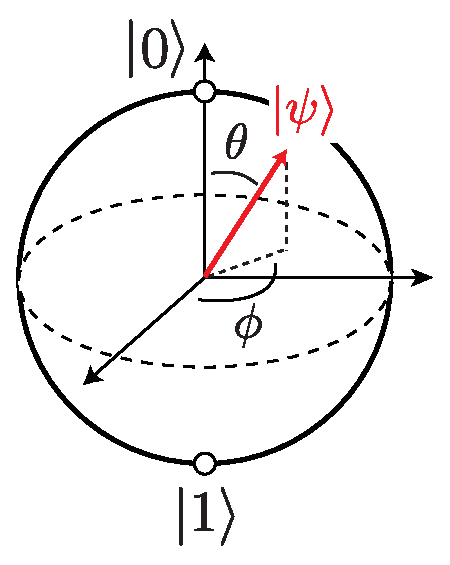
\includegraphics[width=0.5\columnwidth]{FIGURES/FIGURE_2}
\end{center}
\caption{Bloch sphere representation of a qubit.}\label{BS}
\end{figure}
Single qubit gate operations are represented by $2\times2$ unitary matrices and can be interpreted as deterministic rotations of the Bloch vector on the surface of the sphere. Thus, while $\phi$ has no impact on measurement results, it does impact the effect of gate operations.

%The computational unit in an $N$-qubit quantum computer is its $2^N$-length complex state vector,$|\psi\rangle$, and computation consists of unitary operations applied this vector (i.e., $|\psi^\prime\rangle=\hat{U}|\psi\rangle$). As such, these  operators are described by unitary matricies of dimension $2^N\times2^N$. It can be shown that an arbitrary unitary operator can be constructed from a set of single qubit gate operators and a single two-qubit operator~\cite{nielsen2002quantum}. Accordingly, such a library of operations is referred to as universal for quantum computing.
To explain how single qubit gate operations are enabled by the physics of quantum mechanics, we begin by pointing out that a qubit is a quantum mechanical object and, as such, obeys the time-dependent Schr\"odinger equation~\cite{sakurai1995modern},
\begin{equation}
\frac{\partial}{\partial{t}}|\psi\left(t\right)\rangle=-\frac{j}{\hbar}\hat{\mathrm{H}}|\psi\left(t\right)\rangle,
\end{equation}
where $\hbar$ is the reduced Planck's constant and $\hat{\mathrm{H}}$ is the Hamiltonian (total energy) operator, which, for a single qubit, is a $2\times2$ matrix. Since the time-evolution of the qubit state is solely determined by its Hamiltonian, deterministic control of the state of a quantum system requires the ability to systematically enable and disable components of the system's Hamiltonian. In Section~\ref{xmon_control}, we explain how this is carried out for transmon qubits. However,  first we describe these devices.

%It can be shown that single qubit gates can be decomposed into rotations about the $X$, $Y$, and $Z$ axes in the Bloch sphere picture of the qubit state ({\color{red}describe earlier}).  

\subsection{The Flux-Tunable Transmon Qubit}
A schematic diagram of a flux-tunable transmon qubit, complete with XY-drive, Z-drive, and readout ports is shown in Fig.~\ref{XMON}. The intrinsic qubit consists of capacitor $C_\text{Q}$ in parallel with a Josephson junction loop. A Josephson junction is a superconducting tunnel junction and can be thought of as a nonlinear inductance of the form $L_\text{J}=L_\text{J0}/\cos\left(2\pi\Phi/\Phi_\text{0}\right)$, where $\Phi=\int{}v_\text{JJ}\mathrm{dt}$ is the flux \CR{across} the junction, $\Phi_\text{0}=h/2q$ is the flux quanta, $h$ is Planck's constant, $q$ is the charge of an electron, $L_\text{J0}=\Phi_\text{0}/2\pi{}I_\text{C}$, and $I_\text{C}$ is the critical current of the junction and is proportional to junction area~\cite{kadin1999introduction}. A Josephson junction loop, or \CR{superconducting quantum interference device (SQUID)}, can be thought of as a composite Josephson junction, with flux-tunable critical current, $I_\text{C,SQUID}=2I_\text{C0}\left|\cos\left(\pi\Phi_\text{E}/\Phi_0\right)\right|$, where $I_\text{C0}$ is the critical current of each of the (identical) junctions and $\Phi_\text{E}$ is the external flux used to tune the effective critical current~\cite{tinkham2004introduction}. As such, the flux-tunable transmon qubit can be thought of as a frequency-tunable non-linear LC resonator. %Finally, a common perturbation to the tranmon qubit is to replace the single Josephson junction with a Josephson junction loop, or SQUID, which behaves as a flux-tunable nonlinear inductance.
\begin{figure}[bt!]\begin{center}
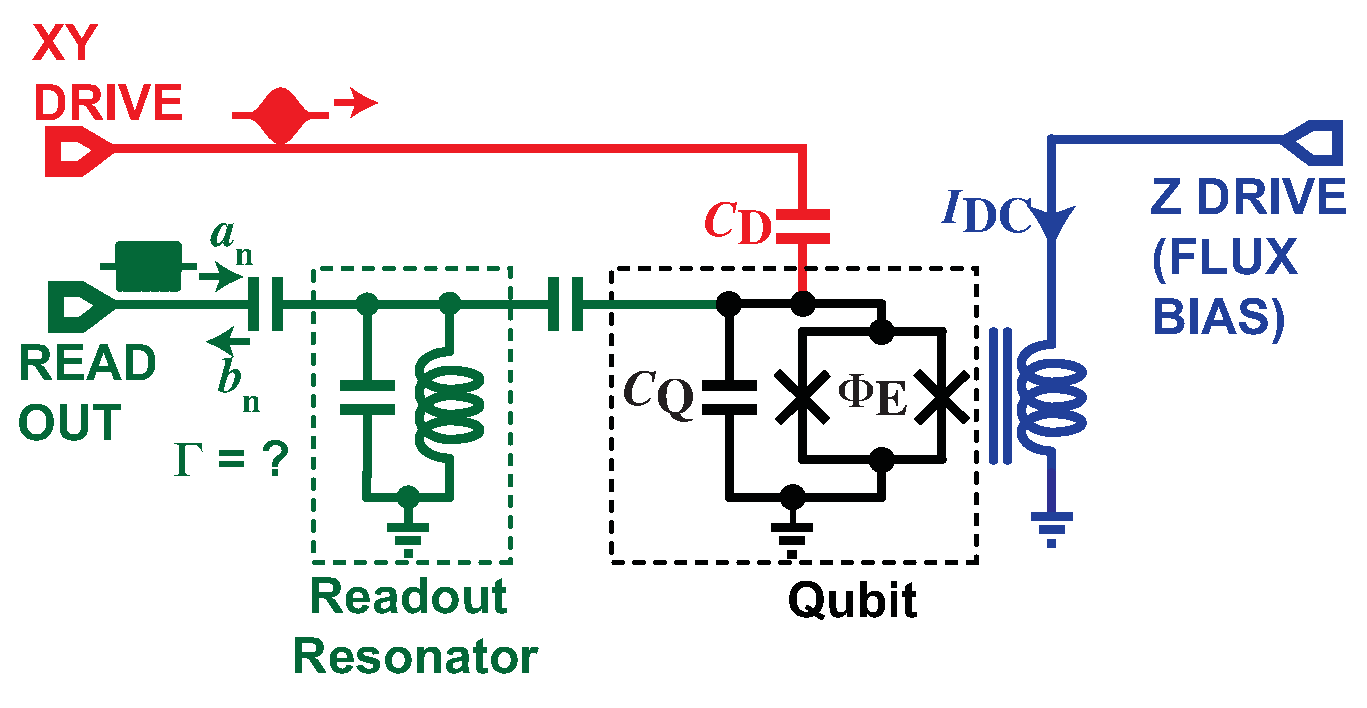
\includegraphics[width=\columnwidth]{Figures/FIGURE_3}
\end{center}
\caption{Schematic diagram of transmon qubit including XY drive, Z drive, and readout ports. The ``X'' symbols represent Josephson junctions\CR{.} The XY drive line is used to induce rotations of the qubit state about an axis in the XY plane of the Bloch sphere, the Z drive is used to control the qubit frequency (useful for two qubit gates, which are beyond the scope of this article), and the readout line is used to perform projective measurements of the qubit state.}\label{XMON}
\end{figure}

If cooled to temperatures such that thermal population of the non-linear resonator is suppressed, a transmon behaves quantum mechanically. For typical qubit frequencies in the vicinity of 5\,GHz, the effective photon temperature ($T_\text{Photon}=hf/k$) is approximately 250\,mK. As such, these devices are \CR{usually} cooled to the 10\,mK range to ensure that thermal excitations are sufficiently suppressed\footnote{This may make it seem advantageous to operate at much higher frequencies to ease the challenges associated with cryogenic cooling. However, this introduces new challenges, including decreased coherence time and more challenging specifications for the control electronics.}. 

The eigenenergies of a transmon can be found from the Hamiltonian of the isolated qubit~\cite{koch2007charge}:
%\begin{equation}
%\hat{H}=\left[\begin{array}{cccc}E_\text{0}&0&0&\cdots\\0&E_\text{1}&0&\cdots\\0&0&E_\text{2}&\cdots\\\vdots&\vdots&\vdots&\ddots\end{array}\right],
%\end{equation}
%where 
\begin{equation}
E_\text{n}\approx\hbar\omega_\text{0}\left(n+\frac{1}{2}\right)-\frac{E_\text{C}}{12}\left(6n^2+6n+3\right).\label{En}
\end{equation}
Here, the index $n$ is an integer greater than or equal to zero, $\omega_\text{0}=1/\sqrt{L_\text{J0}C_\text{Q}}$, and $E_\text{C}=q^2/2C_\text{Q}$ is the energy required to add one electron to the charge on the capacitor. %The first term is that of a linear resonator operating in the quantum in the quantum mechanical regime (i.e., at temperatures where $kT\ll{}\hbar\omega_\text{0}$)
The corresponding energy diagram appears in Fig.~\ref{EnergyDiagram}.  In contrast to the ideal qubit described above, a transmon has many energy levels. As such, care must be taken to ensure that only the lowest two energy levels are occupied. Since it is only possible to populate higher levels if the $|2\rangle$ state is already populated, we will constrain our control signals such that the $|2\rangle$ state is not populated and neglect higher levels in the following discussion.

\begin{figure}
\begin{center}
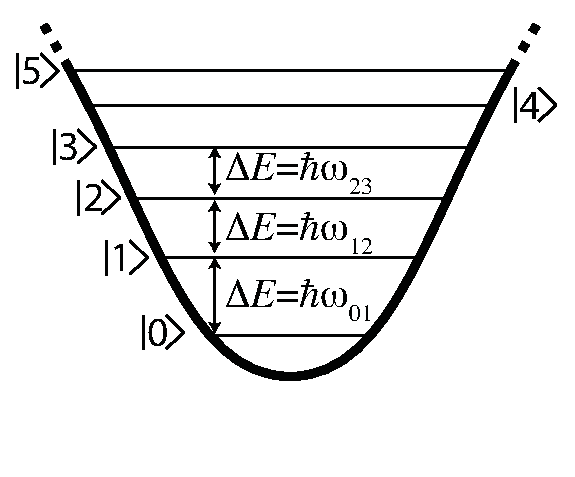
\includegraphics[width=0.6\columnwidth]{Figures/FIGURE_4}
\end{center}
\caption{Energy diagram for transmon qubit. The non-linearity of the Josephson junction creates anharmonicity.}\label{EnergyDiagram}
\end{figure}
The XY drive port shown in Fig.~\ref{XMON} can be used to excite state transitions. The excitation frequencies corresponding to the first two transitions can be determined directly from Equation (\ref{En}):
\begin{equation}
\omega_\text{01}=\frac{E_1-E_0}{\hbar}=\omega_0-E_\text{C}/\hbar
\end{equation}
and 
\begin{equation}
\omega_\text{12}=\frac{E_2-E_1}{\hbar}=\omega_0-2E_\text{C}/\hbar
\end{equation}
From this, we can determine the anharmonicity, or difference between the $\omega_\text{12}$ and $\omega_\text{10}$ transitions:
\begin{equation}
\eta=\omega_{12}-\omega_{01}=-E_\text{C}/\hbar=-\frac{q^2}{2\hbar{}C_\text{Q}}.
\end{equation}
This metric is significant since it bounds the spectral width of microwave excitation pulses, and hence sets a minimum duration for XY gate operations. 
Ideally, the anharmonicity (or qubit nonlinearity) would be as large as possible in order to enable fast gates. However, there is a trade-off, as larger capacitances help to suppress decoherence due to $1/f$ charge noise~\cite{koch2007charge}. Typical values for the magnitude of $\eta/2\pi$ are in the 150--350\,MHz range, with the highest coherence time devices having values towards the lower end of this range.
%It is important to note that the stronger the non-linearity, the 


%The resonator frequency depends on the state of the qubit - \omega_{r,|0>} when the qubit is in |0) and \omega_{r,|1>} when the qubit is in |1). If the resonator is driven in between \omega_{r,|0>} and \omega_{r,|1>}, the phase of the reflected signal depends on the qubit state.
\CR{The Z drive port provides control of the qubit frequency via an externally applied current. This enables several important operations: control of the qubit frequency~\cite{majer2007coupling}, two-qubit interactions (by bringing close in frequency)~\cite{martinis2014fast}, and qubit initialization~\cite{chen2018metrology}. In the context of this paper, we use the Z line to set the qubit frequency and perform initialization. }

A projective measurement of the transmon state can be accomplished through a reflection~\CR{\cite{PhysRevLett.94.123602} or transmission~\cite{blais2004cavity}} measurement of an ancillary linear resonator that is capacitively coupled to the qubit (see Fig.~\ref{XMON}). The coupling between the readout resonator and the qubit will cause a dispersive frequency shift of the readout resonator up or down in frequency if the qubit collapses to its $|0\rangle$ or $|1\rangle$ state, respectively. If the readout resonator is interrogated at the average of these two frequencies, the dispersive frequency shift will produce a state-dependent phase shift on the interrogation signal, which can be detected and used to determine the state of the qubit.
\subsection{XY Control of a Transmon}\label{xmon_control}
%The Hamiltonian of a driven transmon qubit can be written in the rotating frame of the drive signal as~\cite{xx}. 
Assuming a voltage drive referenced to the input of $C_\text{D}$ and of the form 
\begin{equation}
v_\text{D}\left(t\right)=a(t)\sin\left(\omega_\text{D}t+\left(\pi-\phi_\text{D}\right)\right),
\end{equation}
the Hamiltonian of the driven circuit in the rotating frame of the drive signal\footnote{This is similar to a baseband analysis. Here, we have rotated the coordinate system at the carrier frequency to remove dynamics and have assumed that higher frequency components will average out through the integration that occurs when the Schr\"odinger equation is solved.} can be written~\cite{motzoi2009simple}
\begin{equation}
\hat{\mathrm{H}}_\text{D}\approx{}g\frac{a\left(t\right)}{2}\left(\cos\left(\phi_\text{D}\right)\hat{\sigma}_\text{X}+\sin\left(\phi_\text{D}\right)\hat{\sigma}_\text{Y}\right)-\frac{\hbar\Delta\omega}{2}\hat{\sigma}_\text{Z},
\end{equation}
where $g=\left(C_\text{D}/C_\text{Q}\right)\sqrt{\hbar/2Z_\text{Q}}$ is the drive coupling strength, $Z_\text{Q}=\sqrt{L_\text{J0}/C_\text{Q}}$ is the qubit impedance, $\Delta\omega=\omega_\text{D}-\omega_\text{0}$ is the offset in drive frequency from the resonant frequency of the qubit, and
\begin{equation}
\hat{\sigma}_\text{X}=\left[\begin{array}{cc}0&1\\1&0\end{array}\right],~\hat{\sigma}_\text{Y}=\left[\begin{array}{cc}0&-j\\j&0\end{array}\right],~\hat{\sigma}_\text{Z}=\left[\begin{array}{cc}1&0\\0&-1\end{array}\right]
\end{equation}
are the Pauli spin matrices. 

It can be shown that this Hamiltonian produces a time evolution corresponding to a rotation of the qubit state about a vector%~\cite{who} 
\begin{equation}
\left[\begin{array}{c}n_\text{x}\\n_\text{y}\\n_\text{z}\end{array}\right]=\frac{1}{\sqrt{g^2a^2\left(t\right)+\hbar^2\Delta\omega^2}}\left[\begin{array}{c}ga\left(t\right)\cos\left(\phi_\text{D}\right)\\ga\left(t\right)\sin\left(\phi_\text{D}\right)\\-\hbar\Delta\omega\end{array}\right],\label{rabiaxis}
\end{equation}
and at a frequency %{\color{red}Check}
\begin{equation}
\omega_\text{r}=\frac{\sqrt{g^2a^2(t)+\hbar^2\Delta\omega^2}}{\hbar}.\label{rabifreq}
\end{equation}
%\begin{equation}
%\hat{H}=\hbar\omega_\text{r}\left[\begin{array}{cccc}%1/2&0&0&\cdots\\0&3/2&0&\cdots\\0&0&5/2&\cdots\\\vdots&\vdots&\vdots&\ddots\end{array}\right]-E_\text{C}\left[\begin{array}{cccc}1/4&0&0&\cdots\\0&5/4&0&\cdots\\0&0&11/4&\cdots\\\vdots&\vdots&\vdots&\ddots\end{array}\right]\label{driven}
%\end{equation}
Referring to equations (\ref{rabiaxis}) and (\ref{rabifreq}), we can identify three distinct control knobs, $a\left(t\right)$, $\phi_\text{D}$, and $\Delta\omega$. Moreover, it is apparent that $\Delta\omega$ affects the Z component of the rotation axis, whereas the other two degrees of freedom affect its XY projection.
\begin{figure}[bt!]\begin{center}
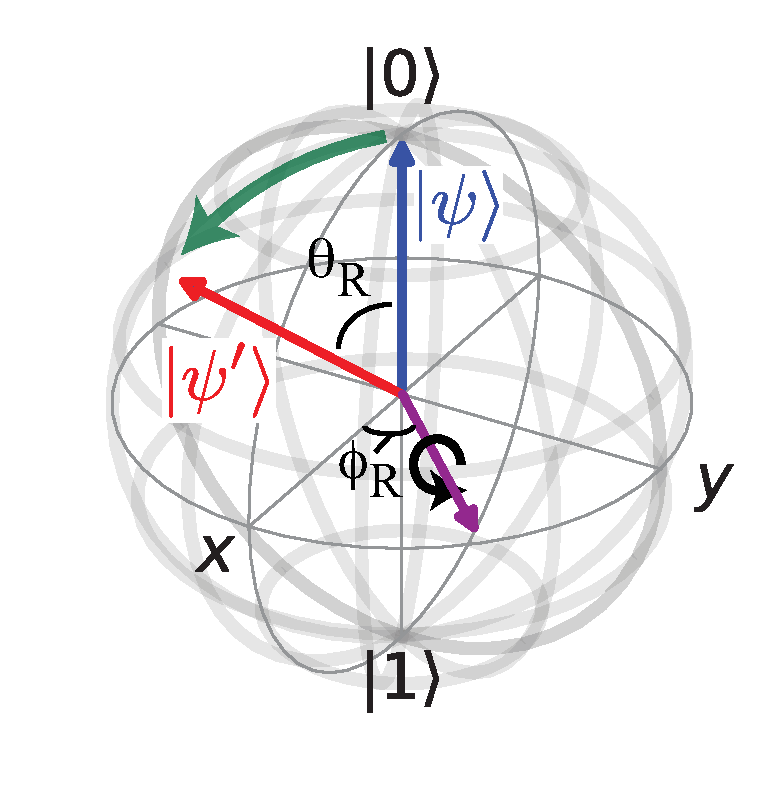
\includegraphics[width=0.6\columnwidth]{Figures/FIGURE_5}\end{center}
\caption{Definition of rotation angles, $\theta_\text{R}$ and $\phi_\text{R}$}
\label{rotatefig}
\end{figure}

Since it is desirable to only induce rotations about an axis in the XY plane of the Bloch sphere (Z rotations can be carried out in software~\cite{mckay2017efficient}), the qubit should nominally be driven on resonance\footnote{It should be noted that the more complete description including $\Delta\omega$ above allows describing the behavior that occurs if the drive signal is slightly detuned from the qubit frequency.} ($\Delta\omega=0$). In this case, as defined in Fig.~\ref{rotatefig}, the axis of rotation is defined by the carrier phase, $\phi_\text{R}=\phi_\text{D}$, and the angle of rotation is proportional to the integrated envelope amplitude
\begin{equation}
\theta_\text{R}=\frac{g}{\hbar}\int_{t_0}^ta\left(t^\prime\right)\mathrm{dt^\prime}.\label{rotate}
\end{equation}


A block diagram of a standard control and readout system appears  in Fig.~\ref{stdXY} with the XY control portion highlighted. The XY signals are generated using a pair of 1 \CR{GS}/s 14-bit DACs whose outputs drive the \CR{in-phase and quadrature} ports of an IQ mixer. Single sideband (SSB) mixing is typically employed, with LO and RF signals in the 4--8\,GHz frequency range. \CR{To reduce the thermal noise floor well below the effective temperature of a photon at the qubit frequency---required to suppress thermal excitations---}the upconverted output of the SSB mixer is heavily attenuated at both the 3-K and 10-mK stages of the cryogenic system\footnote{\CR{Attenuation is distributed across temperatures to minimize power dissipation at 10\,mK while still reducing the thermal noise floor sufficiently.}}.  In the remainder of the paper, we consider simplifying and integrating this system in a manner such that it can be placed on the 3-K stage of the cryostat.

\begin{figure}[bt!]
\begin{center}
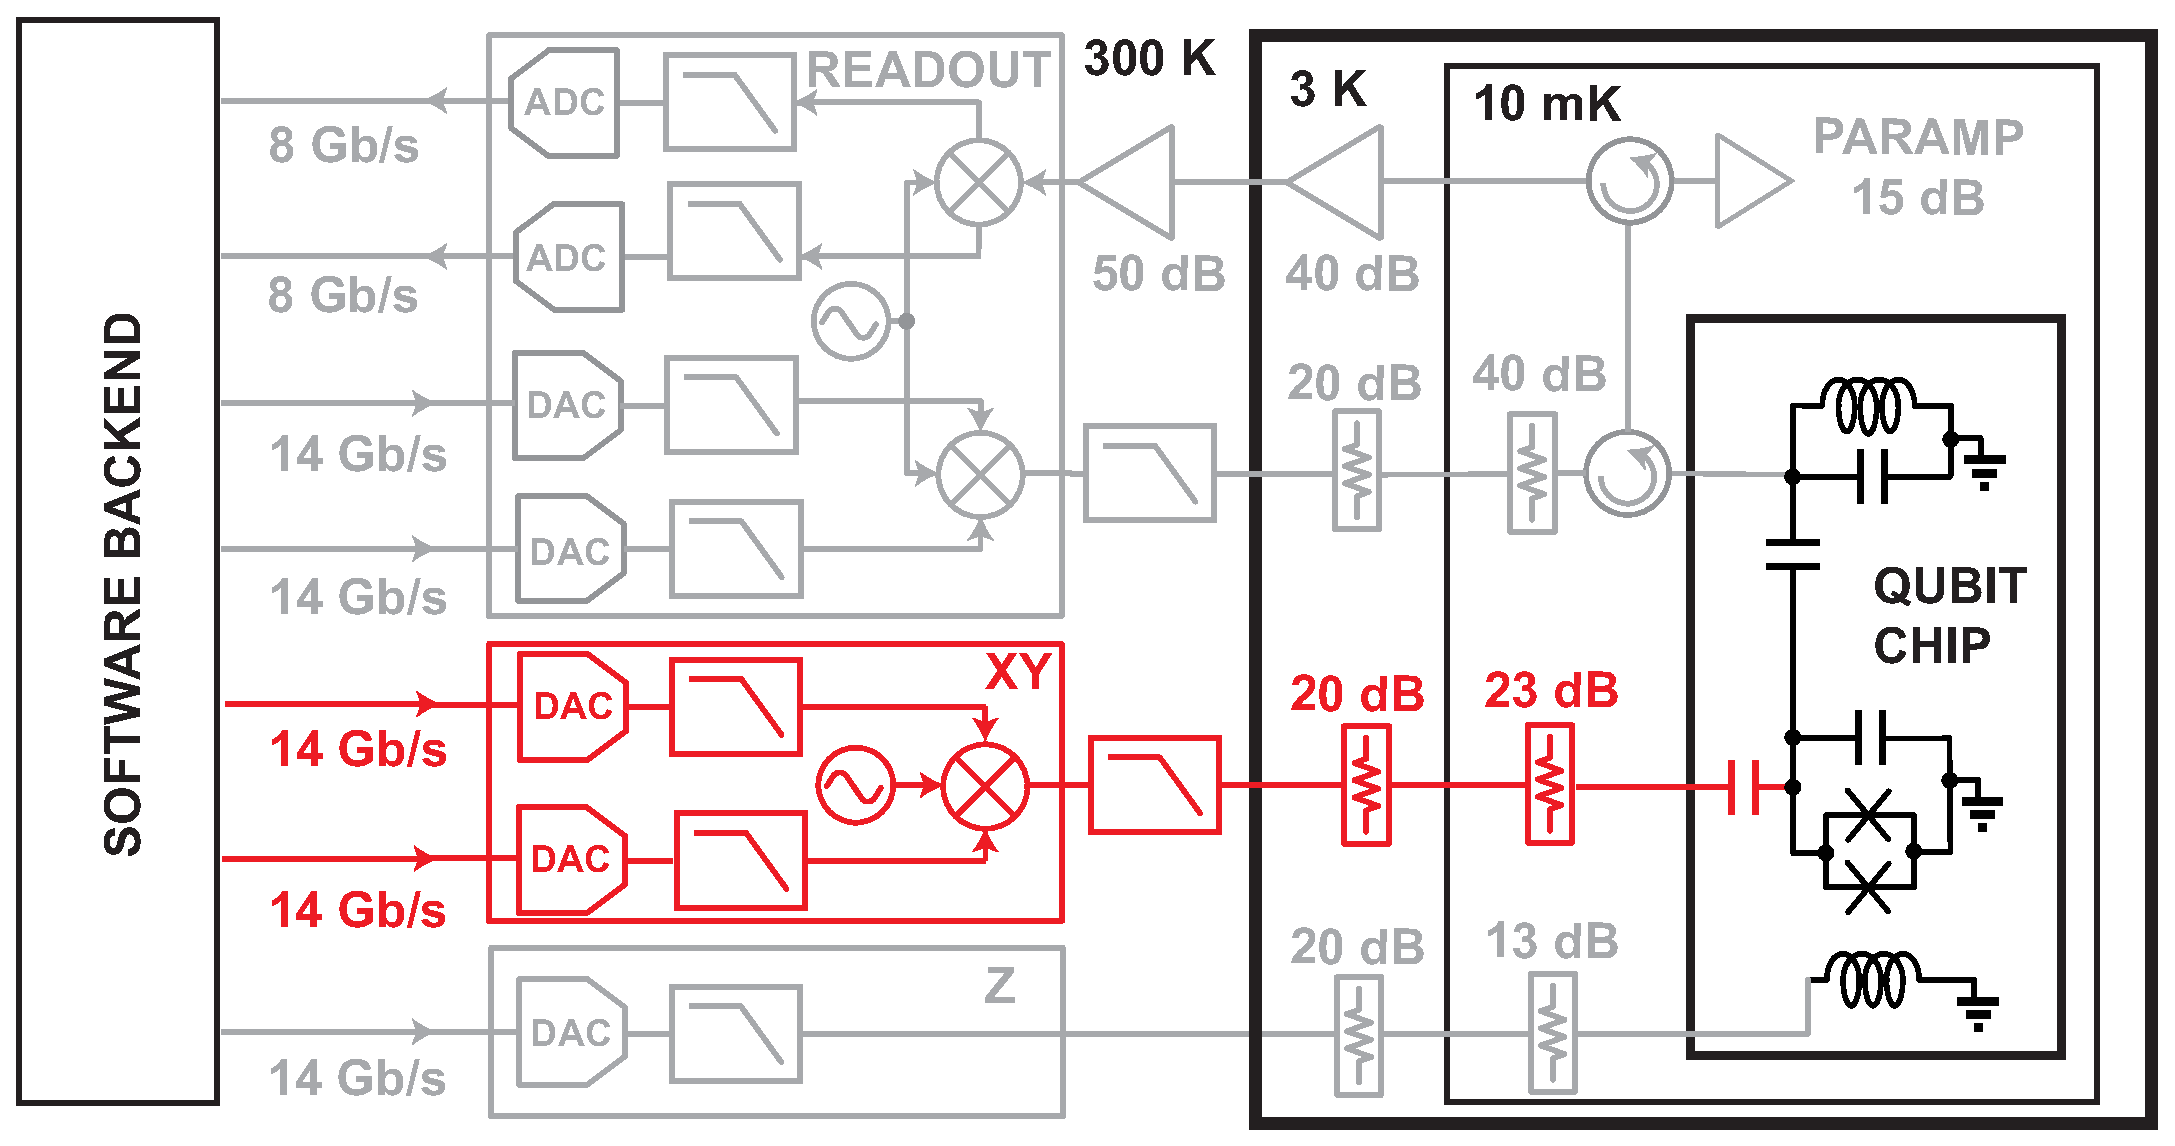
\includegraphics[width=\columnwidth]{Figures/FIGURE_6}
\end{center}
\caption{Block diagram showing standard control and readout hardware, with XY control hardware highlighted.}\label{stdXY}
\end{figure}
\section{XY Controller Requirements}\label{requirements}
Techniques to accurately control and measure the state of a quantum processor with on the order of a million qubits will be required to enable fault tolerant quantum computing~\cite{fowler2012surface}. As a first step towards such a quantum control and measurement system, we consider the implementation of a  cryogenic pulse modulator IC, optimized to generate XY control signals. Here we summarize some of the key specifications \CR{that this circuit must eventually meet if it is to displace today's rack mount control systems}. %Unless stated otherwise, {\color{red}in the discussion below, we assume that multiplexing of control signals is not feasible.}

\subsection{\CR{Ambient} Temperature}
We first consider the \CR{ambient} temperature at which to thermalize the quantum controller, as this is critical in driving other specifications. On the one hand, it is desirable to place the controller as close as possible to the quantum processor so as to minimize interconnects. In fact, if there were no other considerations, it would be appropriate to co-integrate the classical control with the quantum chip. In hopes of making this a reality, researchers are currently exploring both 3D packaging approaches~\cite{rosenberg20173d} and integrated control and readout architectures~\cite{leonard2019digital,opremcak2018measurement,mcdermott2018quantum}.

However,  as discussed above, superconductive quantum processors must be thermalized to temperatures in the range of 10\,mK. Unfortunately, the efficiency of cryocoolers is fundamentally limited by the laws of  thermodynamics to $\eta\le{}T_\text{BASE}/\left(T_\text{A}-T_\text{BASE}\right)$, where $T_\text{BASE}$ and $T_\text{A}$ are the base and room temperatures, respectively~\cite{kittel1969thermal}. So, the efficiency in removing heat at 10\,mK cannot be more than about 0.003\%. In reality, the efficiency of commercial dilution refrigerators used for cooling to 10\,mK is orders of magnitude lower than the theoretical Carnot efficiency. In fact, typical systems can handle less than 15$\,\mu$W at 10\,mK, despite drawing more than 10\,kW of wall power~\cite{oxford,pt420}. As such, thermalization of CMOS integrated control electronics to the same stage as the quantum IC is not viewed as a viable approach.

At the other extreme, we could consider placing the quantum controller at room temperature, as done today. The advantage here is that power consumption of the electronics is not critical and existing electronics could be miniaturized and scaled. However, scaling of the interconnects connecting the room temperature electronics to the 10\,mK stage is very challenging, as these lines must be able to support microwave transmission with high isolation while presenting as low of a thermal load as possible. As such, it is not believed to be scalable to the levels required to control a quantum processor with a million or more qubits. 
 
A more tractable solution is to thermalize the control electronics in the range of 3-to-4\,K and use superconductive transmission lines to couple the control signals down to the 10\,mK stage~\cite{ hornibrook2015cryogenic,CharbonISSCC}. By using superconducting interconnects, it is possible to achieve excellent electrical and thermal performance in a small cross sectional area~\cite{tuckerman2016flexible}. Below, we will assume that the quantum control electronics are thermalized in the range of 3-to-4\,K.
\subsection{Power Consumption}
While much higher than at 10\,mK, the power handling capability of the 4\,K stage of a typical closed-cycle refrigeration system is still limited.  For near-term systems, which will employ standard pulse-tube cryocoolers, the total dissipation at 4\,K will be limited to just 2\,W at 4\,K~\cite{cryomech}. As this power budget must include any thermal load associated with cabling, the actual power available for electronic consumption is lower. As such, a reasonable near term power budget for the control and readout electronics is 1\,W.

For a scaled system, one could envision building a much larger refrigerator and employing more advanced cooling techniques. For instance, helium \CR{refrigeration systems} can be used to increase the capacity to around  1\,kW~\CR{\cite{linde}}, or  about 1\,mW/qubit at the million qubit level. As this power consumption must be shared between any incoming cabling (from 300\,K), Z-control electronics, and the readout electronics (which can be multiplexed by 5-10x), a reasonable long term limit for the dissipation of the \CR{XY} control electronics is 250\,$\mu$W per qubit. For this proof of concept work, which is being carried out without cryogenic simulation models, we relax this specification by a factor of ten to 2.5\,mW, with the expectation that the power consumption can be further optimized in a future design. 
\subsection{Frequency Range}
Typical transmon qubits have transition frequencies in the 4--8\,GHz frequency range. As such, we seek to cover this full band with our initial prototype device. However, it may be desirable for a future device to only operate over some sub-set of this frequency range.
\subsection{Gate Fidelity and Error Rates}
The remainder of the specifications are all performance related and, as such, a metric to benchmark performance is required. Fidelity and error rates provide such metrics. Gate fidelity is a measure of how close the effect of an applied gate is to that of the desired unitary and can be limited by a number of factors including control errors, noise, decoherence, etc. Formally, we can define the gate fidelity of a single qubit gate, averaged over all pure input states as~\cite{pedersen2007fidelity}
\begin{equation}
\mathscr{F}_\text{G}\equiv\frac{\Tr\left\{U_\text{Ideal}^\dagger{}UU^\dagger{}U_\text{Ideal}\right\}+\left|\Tr\left\{U_\text{Ideal}^\dagger{}U\right\}\right|^2}{6}.
\end{equation}
The first term, $\Tr\left\{U_\text{Ideal}^\dagger{}UU^\dagger{}U_\text{Ideal}\right\}$ evaluates to two in the case that the realized operator is unitary, but is smaller in the case where the matrix is not unitary due to matrix truncation (e.g., if there is leakage to the $|2\rangle$ state). 
In a computation, the average error per step is simply $1-\mathscr{F}_\text{G}$.

The degree of redundancy required for fault tolerant quantum computing is strongly dependent upon error rates~\cite{fowler2012surface}. In order to reduce this to practical levels, the error rates should be \CR{minimized}. Here, we \CR{provide specifications corresponding to an overall error rate of 0.01\%, which is slightly better than the state of the art~\cite{barends2014superconducting}. To achieve this, individual error contributors should be an order of magnitude lower.}

\subsection{Noise on the Drive Line}
Noise at the qubit transition frequency causes decoherence. An available noise power spectral density of $S_\text{a}\left(f_\text{01}\right)=kT_\text{e}$ at the drive port at frequency $f_\text{01}$ leads to transitions between the $|0\rangle$ and $|1\rangle$ states at a rate~\cite{clerk2010introduction}
\begin{equation}
R_{\uparrow\downarrow}=2\pi\frac{T_\text{e}\left(f_\text{01}\right)}{T_\text{Photon}}\Delta{f},
\end{equation}
where $\Delta{f}=f_\text{0}/Q_\text{D}$, $Q_\text{D}=\left(C_\text{Q}/C_\text{D}\right)^2\left(Z_\text{Q}/Z_\text{0}\right)$ is the quality factor of the qubit due to the drive circuit, $T_\text{Photon}=\hbar\omega_\text{01}/k$ is the effective temperature of a photon at the qubit frequency, and $Z_\text{0}$ is impedance of the drive port. The noise spectral density $S_\text{a}=kT_\text{e}$ must be kept low enough such that $R_{\uparrow \downarrow}$ is less than other decoherence channels in the system, such as losses from materials imperfections. This usually means ensuring that the noise temperature seen looking back into the drive line is kept well below the effective temperature of a photon at the drive frequency. As such, it is important both to include attenuation at 10\,mK on the drive line and also to minimize noise generated by the XY controller. \CR{Any excess noise generated by the quantum controller (beyond that of a thermal source) will require excess attenuation. As such, this noise should be minimized.}
%\subsection{Gate Time}
% Assuming the gate time ($T_\text{G}$) is much less than the coherence time ($T_\text{1}$), then the work case error rate due to decoherence is simply
%\begin{equation}
%\epsilon_\text{T1}\le{}1-e^{-T_\text{G}/T_\text{1}}\approx\frac{T_\text{G}}{T_\text{1}}
%\end{equation}
%As such, it is desirable to 
\subsection{Spectral Content}
Also related to gate fidelity is the spectral content of the qubit drive signal. Due to the finite coherence time of a qubit (on the order of 10-to-100\,$\mu$s for transmon qubits) fast gates are desired. However, due to the finite separation between the $\omega_\text{01}$ and $\omega_\text{12}$ transition frequencies, it is important to ensure that the drive signal does not introduce leakage to higher order levels. \CR{Errors due to spectral leakage can be estimated as the ratio of energy in a pulse at the undesired transition to that at the qubit frequency~\cite{steffen2003accurate}. Reducing this error rate to $10^{-5}$ requires suppressing energy at the $\omega_\text{12}$ transition by 50\,dB. As such, one has to carefully balance the trade-off between speed and leakage when selecting pulse waveforms}. Typical pulse envelopes include Gaussian and raised cosine shapes and advanced techniques such as derivative removal by adiabatic gate (DRAG) are used regularly to further reduce the pulse duration beyond what can be achieved using envelope shaping alone~\cite{motzoi2009simple,gambetta2011analytic}. In this work, we limit our pulse generation capabilities to simple symmetric pulses without derivative compensation. 
%\cite{twostatemartinis}


\subsection{Amplitude Control}
The drive amplitude sets the range of rotations that can be carried out for a given pulse duration. As discussed in Section~\ref{xmon_control}, a drive pulse on resonance with the qubit produces a rotation proportional to the integrated envelope amplitude (see Equation~(\ref{rotate})). The largest rotation required in a practical quantum algorithm is a $\pi$-pulse, \CR{which induces a 180$^\circ$ rotation on the Bloch sphere}. For a raised cosine envelope, the  peak amplitude required to achieve this rotation is
\begin{equation}
A_{\text{PK},\pi}=2\pi\frac{\hbar}{g\tau_\text{G}},
\end{equation}
\CR{where $\tau_\text{G}$ is the gate duration and is typically between 10 and 30\,ns.} For typical values of $g$, the required peak amplitude for a 15\,ns pulse is on the order of 100\,$\mu$V (peak available power of -76\,dBm). 

\CR{In general, we want to be able to drive with pulses several times larger to both to carry out rotations well beyond $180^\circ$ and also to enable shorter $\pi$-pulses}. As such, it is desirable that the XY controller be able to drive pulses on the order of 1\,mV at the reference plane of the qubit drive port. The signal \CR{amplitude} at \CR{3\,K} must be about an order of magnitude larger to account for the attenuation on the drive line that is required at 10\,mK to reduce the thermal noise floor. \CR{If the noise floor of the quantum controller is larger than that of a thermal source, the signal amplitude must be increased to account for additional attenuation that is required due to this excess noise.}

Amplitude resolution is also important, since any error in pulse amplitude will translate to an over or under rotation and contribute to gate error rates. An error in a rotation of $\Delta{\theta_\text{R}}$ produces an average error rate of
\begin{equation}
\epsilon_{\Delta{\theta_\text{R}}}\approx{}\frac{\Delta{}\theta_\text{R}^2}{6}.
\end{equation}
To keep error rates due to integrated envelope amplitude errors below $10^{-5}$, it is necessary that XY rotation angles are controlled to better than \CR{$0.45^\circ$}. This means that the integrated $\pi$-pulse amplitude must have an accuracy better than $0.25\%$. \CR{This resolution can be achieved by varying the pulse duration or scaling the envelope amplitude. Here, we take the latter approach.}%A resolution of 11 bits in the integrated envelope amplitude is required to provide the required dynamic range\footnote{It should be noted that this is not the dynamic range that must be achieved on a pulse to pulse basis, but rather what a design should be able to achieve over its entire configuration range. For typical operation, where the largest signal one would apply is a $\pi$-pulse, an order of magnitude lower dynamic range is acceptable.}.
\subsection{Carrier Phase Control}
A carrier phase error of $\Delta\phi_\text{D}$ on an XY gate will lead to a rotation around the wrong axis, resulting in an average gate error rate of 
\begin{equation}
\epsilon_{\Delta\phi_\text{D}}=\frac{2}{3}\Delta\phi_\text{D}^2\sin^2\left(\frac{\theta_\text{R}}{2}\right)\left(1-\frac{\Delta\phi_\text{D}^2}{4}\sin^2\left(\frac{\theta_\text{R}}{2}\right)\right).
\end{equation} 
For small phase errors, it can be shown that the worst case average error rate will occur for $\pi$-pulses. To ensure the contribution of phase to the error rate is below \CR{$10^{-5}$} for all XY rotations, it is necessary that the carrier phase be controlled to better than \CR{$0.22^\circ$}. 

%To understand the procedure of specifying the drive amplitude, we consider a transmon qubit with a capacitively coupled drive, as {\color{red} described...}. When driven on resonance, the drive Hamiltonian for this circuit can be expressed in the rotating frame of the qubit as
%\begin{equation}
%\hat{H}_\text{d}=\alpha\frac{e\left(t\right)}{2}\left[\begin{array}{cc}0&e^{-j\phi_\text{d}}\\e^{j\phi_\text{d}}&0\end{array}\right],
%\end{equation}
%where $\alpha=C_\text{D}\sqrt{\hbar\omega_\text{01}/\left(2C\right)}$ is a constant quantifying the drive coupling. The corresponding time evolution operator is 
%\begin{equation}
%\hat{U}_\text{XY}\left(t,t_\text{0}\right)=\left[\begin{array}{cc}\cos\left(\frac{\Theta}{2}\right)&-j\sin\left(\frac{\Theta}{2}\right)e^{-j\phi_\text{d}}\\\\-j\sin\left(\frac{\Theta}{2}\right)e^{j\phi_\text{d}}&\cos\left(\frac{\Theta}{2}\right)\end{array}\right],
%\end{equation}
%where 
%\begin{equation}
%\Theta=\frac{\alpha}{\hbar}\int_{t_0}^{t}e\left(t^\prime\right)\mathrm{d}t^\prime.
%\%end{equation}
%There are a couple things to note here. First, the  
\begin{table*}
\begin{center}
\caption{Key specifications for cryogenic XY controller}\label{perfspecs}
\begin{tabular}{lrrrrrrrrr}
\toprule
&Amb. Temp.&RF Frequency&Envelope&Env. Amp&Pulse Duration&Amp. err.&Phase err&Inst. Set&AC+DC Power\\
\midrule
Prototype Goal&\CR{3}\,K&4-to-8\,GHz&Symmetric&$>$10\,mV&10-to-30\,ns&$<0.15\%$ &\CR{$<0.22^\circ$}&16 (4-bit)&$<$2.50\,mW\\
Long-term Goal&\CR{3-to-4.2\,K}&TBD&DRAG&$>1\,$mV&$<$10\,ns&$<0.15\%$&\CR{$<0.22^\circ$}&TBD&$<$250\,$\mu$W\\
\bottomrule
\end{tabular}
\end{center}
\end{table*}


\subsection{ON/OFF Ratio}
\label{ONOFF}
\CR{Carrier leakage causes initialization errors, reduces gate fidelity, and can lead to measurement errors.} This effect is most significant for direct conversion pulse modulation architectures, for which the leakage tone is on-resonance with the qubit. %In this case, equation~(\ref{driven}) can applied directly if we set the envelope term as, $e\left(t\right)=E_\text{L}$, where $E_\text{L}$ is the leakage amplitude. 
To understand the effect on initialization, we consider the case in which the qubit is reset to the ground state at $t=0$ and idles for a time $\Delta{t}$ prior to being intentionally driven. Such a delay is typical to permit settling of the qubit after initialization. Under this scenario, a leakage tone with amplitude $A_\text{L}$ produces a persistent XY rotation, resulting in a $|1\rangle$ state population due to leakage of $P_\text{L}\left\{|1\rangle\right\}=\sin^2\left(gA_\text{L}\Delta{t}/2\hbar\right)$, which for small enough $A_\text{L}\Delta{t}$ products simplifies to $P_\text{L}\left\{|1\rangle\right\}\approx{}\left(gA_\text{L}\Delta{t}/2\hbar\right)^2$. So, defining the specification for ON/OFF ratio in terms of the peak pulse amplitude required for a $\pi$-pulse ($A_{\text{PK,}\pi}$) and assuming raised cosine pulse shaping, we find
\begin{equation}
R_\text{ON/OFF}\equiv{}\frac{A_{\text{PK},\pi}}{A_\text{L}}\approx{\pi}\frac{\Delta{}t}{\CR{\tau_\text{G}}}\frac{1}{\sqrt{P_\text{L}\left\{|1\rangle\right\}}},\label{ONOFFratio}
\end{equation}
where $P_\text{L}\left\{|1\rangle\right\}$ is the initialization error due to leakage. As a numerical example, if \CR{$\tau_\text{G}=15\,$}ns, achieving an initialization error of 0.01\% with a settling time of 500\,ns requires an ON/OFF ratio of 
80\,dB. \CR{If this specification is met, the corresponding idle gate  error is $10^{-7}$. While an 80\,dB ON/OFF ratio is a stringent specification,} it should be feasible to meet this requirement using modern cancellation techniques due to the narrowband nature of the carrier leakage. \CR{Alternatively, the ON/OFF ratio requirement could be greatly reduced by moving to a SSB pulse generation approach (non-zero IF) or by using Z control to detune the qubit during idling.}

\begin{figure}[bt!]
\begin{center}
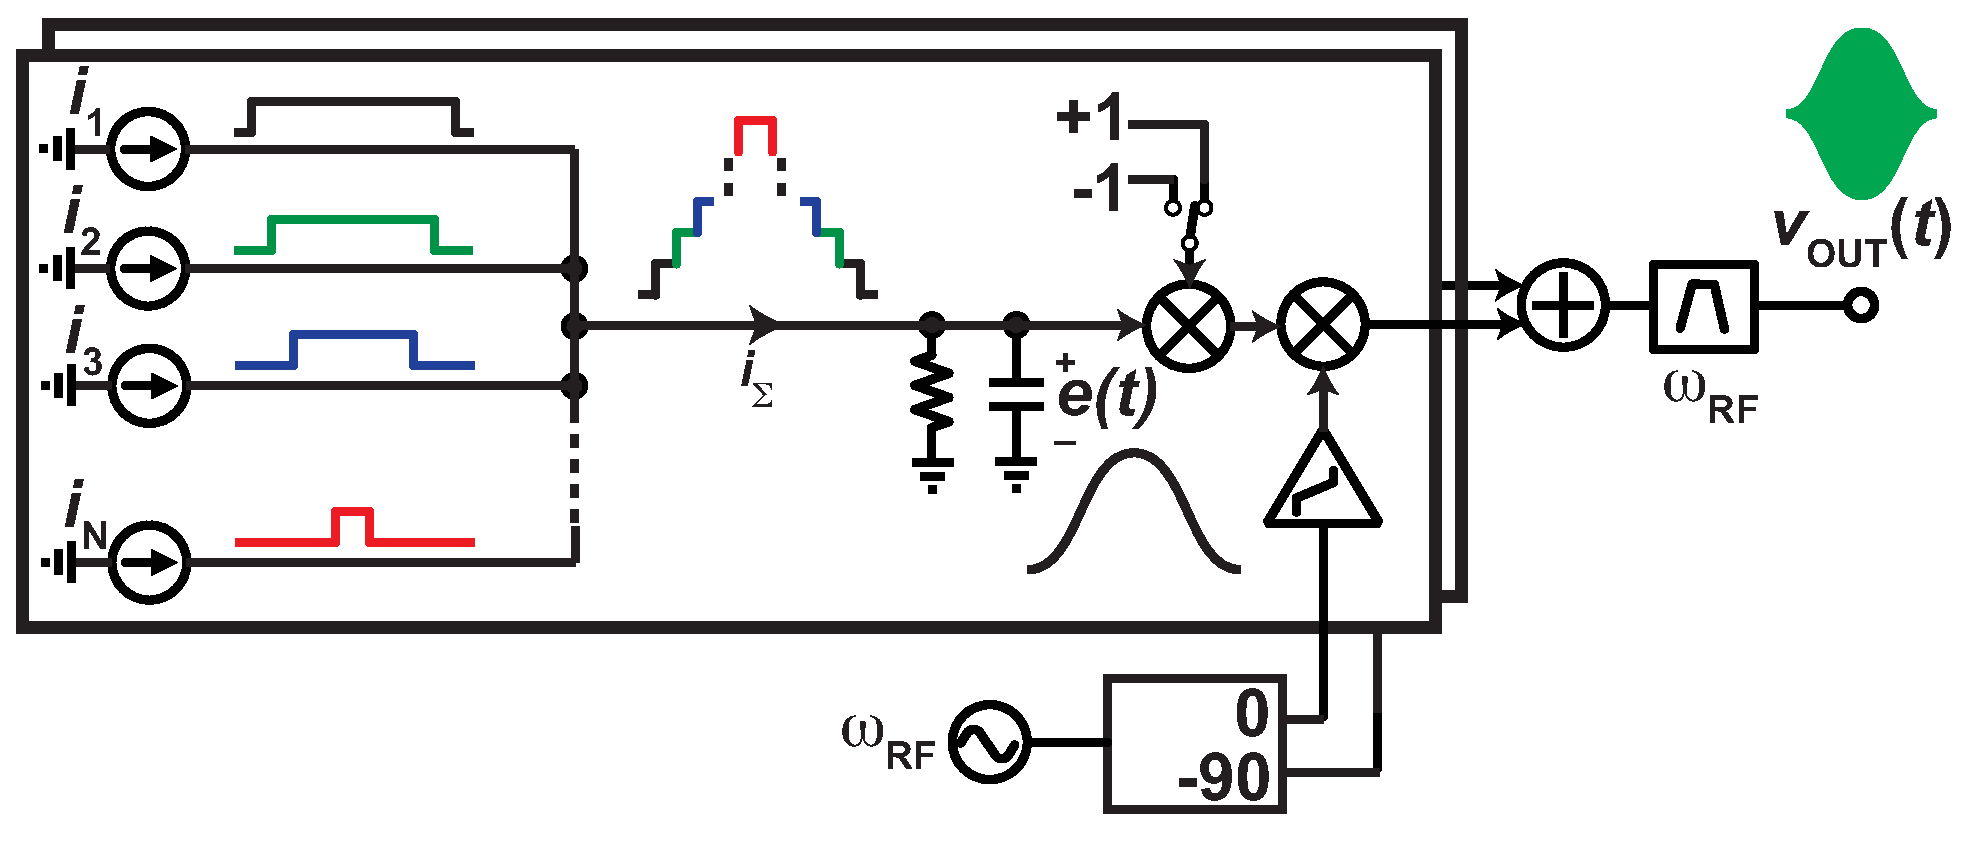
\includegraphics[width=\columnwidth]{Figures/FIGURE_7}
\end{center}
\caption{Block diagram of the proposed pulse generation approach.}
\label{Concept}
\end{figure}

%Another important metric is the $|1\rangle$ state population that is driven by carrier leakage over the course of a coherence time, an upper limit for which can be determined by substituting $T_\text{1}$ for \CR{$\tau_\text{G}$} in equation (\ref{ONOFFratio}). A reasonable limit to this value is 5\% for a typical $T_\text{1}$ value of 20\,$\mu$s. Reaching this value requires a slightly higher ON/OFF ratio of 85\,dB. While this is a stringent specification, it should be feasible to meet this using modern cancellation techniques due to the narrowband nature of the carrier leakage.





\subsection{Summary}
The performance specifications of the XY controller are summarized in Table~\ref{perfspecs}. \CR{It should be noted that a 16-word instruction set has been selected in order to permit the definition of rotations of $\pm{}90^\circ$ and $\pm{}180^\circ$ about the X and Y \CG{axes} as well as to leave space to define a small set of all-microwave Z-gates (rotations about the Z-axis, realized by combining XY gates)}. 

% The degree of these effects depends upon the idle state Hamiltonian of the driven qubit, as expressed in the rotating frame, referenced to the leakage frequency\footnote{This is equivalent to a baseband representation, with respect to }
%\begin{equation}
%\hat{H}_\text{R}=\left[\right],
%\end{equation}
%where... 
%From this, one can determine the corresponding time evolution operator and thus the stray population of the $|1\rangle$ state during idling. A reasonable specification is that the idle $|1\rangle$ state population is below 5\% over a coherence time (corresponding to an infidelity of ...). 

%The significance of this effect depends on the CW frequency leaking out of the quantum controller during idling and is maximized when this leakage is on resonance with the qubit. As such, a direct conversion approach for control signal generation requires a significantly higher ON/OFF ration in comparison with single-sideband modulation approaches. The effect can be quantified through the Hamiltonian, referenced to the rotating frame of the leakage signal. Assuming that the qubit is initialized to the ground state at $t=0$ and that carrier leakage drives only the $0\to1$ transition, 
%\begin{equation}
%P\left\{|1\rangle\right\}|_{T=T_\text{1}}=\frac{\gamma^2}{\gamma^2+\Delta^2}\sin^2\left(\frac{\sqrt{\gamma^2+\Delta^2}}{2}T_\text{1}\right),
%\end{equation}
%where gamma is 

%To ensure that these effects are negligible, we can specify a maximum level of initialization error at the end of a coherence time. 





\section{Circuit Design}
A conceptual block diagram explaining the waveform generation approach appears in Fig.~\ref{Concept}. A vector modulation based architecture has been chosen to enable simultaneous control of the envelope amplitude and carrier phase. Symmetric envelopes are generated using an array of current sources which are sequentially enabled and disabled with the appropriate timing to generate a symmetric staircase of current, as shown in Fig.~\ref{Concept}. The current waveform is then lowpass-filtered to create a smooth envelope. By controlling the individual weights of each of the current-mode sub-DACs, a wide range of symmetric envelopes can be realized. After lowpass filtering, the envelope currents pass through a polarity switch, are up-converted to the carrier frequency, and the two quadratures are then combined to create the output pulse. 


This architecture has been chosen as a trade-off between power consumption, performance, and robustness to the inherent uncertainty associated with designing for operation at 3-K, where foundry design models are currently unavailable. Several research groups are currently investigating the cryogenic performance of nanometer CMOS technology (e.g.,~\cite{incandela2018characterization,beckers2018characterization}) and it is known that threshold voltages, transconductances, and subthreshold \CR{swing} all change with cryogenic cooling. Unfortunately, mismatch is also degraded, particularly in the sub-threshold regime~\cite{mismatch}. A critical feature of the envelope generation approach is guaranteed monotonicity, even if the sub-DACs display non-linearity or non-monotonicity.

A block diagram of the implemented IC appears in Fig.~\ref{chipbd}. The circuit consists of a pair of baseband envelope DACs, which drive a vector modulator. The clock port of the DACs and the LO ports of the vector modulator are buffered to minimize the external RF power required to drive the chip. A small digital memory is incorporated to store configuration parameters and implement a rudimentary 4-bit (\CR{16 word}) XY instruction set. By integrating such an instruction set on-chip, the overall digital I/O rate required to operate the chip is greatly reduced, thereby resulting in a significant savings in power and system complexity. A trigger line is included to initialize a pulse.
\begin{figure}[bt!]
\includegraphics[width=\columnwidth]{Figures/FIGURE_8}
\caption{Block diagram of the cryo-CMOS pulse generator.}\label{chipbd}
\end{figure}
\begin{figure}
\includegraphics[width=\columnwidth]{Figures/FIGURE_9}
\caption{Simplified schematic diagram of one of the envelope DACs.}
\label{EnvD}
\end{figure}

A schematic diagram of one of the envelope DACs appears in Fig.~\ref{EnvD}. The circuit contains a bank of eleven 8-bit current-mode sub-DACs, whose outputs are combined in the current domain and lowpass filtered before being fed to the modulator stage. Each DAC is constructed using a binary-weighted current mirror circuit, with the smallest unit cell being a minimum feature-size transistor. While linearity and monotonicity could be improved by using larger transistors and thermometer coding, respectively, these properties were sacrificed to reduce dynamic power consumption. \CR{A switched current mirror architecture was selected over a current steering one to reduce static power consumption.} The bank of DACs share a common reference current ($I_\text{N}$), \CR{generated by an 8-bit reference DAC implemented as a binary weighted current mirror}. \CR{The reference DAC is} biased from a current source ($I_\text{P}$) which has an additional 6-bits of reconfigurability. The configuration bits for each of the sub-DACs as well as \CR{the reference DAC (generating} $I_\text{N}$) are configured by the sixteen-waveform configuration memory, with the desired waveform  selected by the 4-bit instruction interface ($\mathrm{SEL<0:3>}$). %{\color{red}line here about extra bits}


A current waveform of the form shown in Fig.~\ref{Concept} is generated by enabling each of the 11 current sources in the appropriate sequence. The  enable signals for this operation are generated by the pulse controller shown in Fig.~\ref{EnvD}. The pulse controller is a shift-register based design in which the enable signal propagates through the shift register after a trigger pulse has been detected. To minimize the power consumption of this block, the clock signal is gated such that each flip-flop is only clocked if its output is \CR{scheduled} to transition during a given clock cycle. \CR{The controller produces pulses that are 21 clock cycles long. The circuitry was implemented using a mixture of custom and standard cell components and, to enable pulses as short as 10\,ns, it was optimized to operate at clock frequencies up to 2.1\,GHz. The output of each current-mode DAC is filtered using by a simple RC network that also serves to terminate the IF port of the RF mixer. This network consists of a 500\,$\Omega$ resistor in parallel with a 4-bit binary-weighted capacitor bank with an aggregate capacitance of 9\,pF (enabling cutoff frequencies as low as 35\,MHz).} %The controller was designed to accept clock signals in excess of 2\,GHz and produces pulses that are 21 clock cycles long.     

A schematic diagram of the passive-mixer-based vector modulator appears in Fig.~\ref{vectormod}. A passive mixer has been selected to avoid introducing noise of a non-thermal nature during the mixing process and the circuit has been designed as a trade-off between power consumption and \CR{frequency coverage}. Each LO signal is transformer-coupled to a fully differential gain block which helps to improve common-mode rejection.  The differential output of this cell is further amplified by a standard-cell based pseudo-differential amplifier chain that is sized to drive the mixer \CR{at digital levels. The switching transistors were each implemented as a single $4\times\,1\,\mu$m$\,\times\,30\,$nm transistor. This sizing was chosen as a trade-off between on-resistance (60~$\Omega$) and gate-capacitance (3.5\,fF), as simulated using the room temperature PDK models.} \CR{A 4-bit capacitor bank is incorporated on the pad-side of each input transformer to enable optimum coupling over the 4--8\,GHz frequency range.} \CR{The LO paths were optimized to be driven with LO signals below 50\,$\mu$W and  simulation using room-temperature models predicts a jitter contribution of less than 100\,fs (integrated from 50\,kHz to 50\,MHz), corresponding to a phase error contribution below $0.22^\circ$ RMS for a 5.6\,GHz LO. As this is dominated by the broadband noise floor, the jitter contribution is expected to be significantly lower when the device is operated at cryogenic temperatures}. 
\begin{figure}[bt!] 
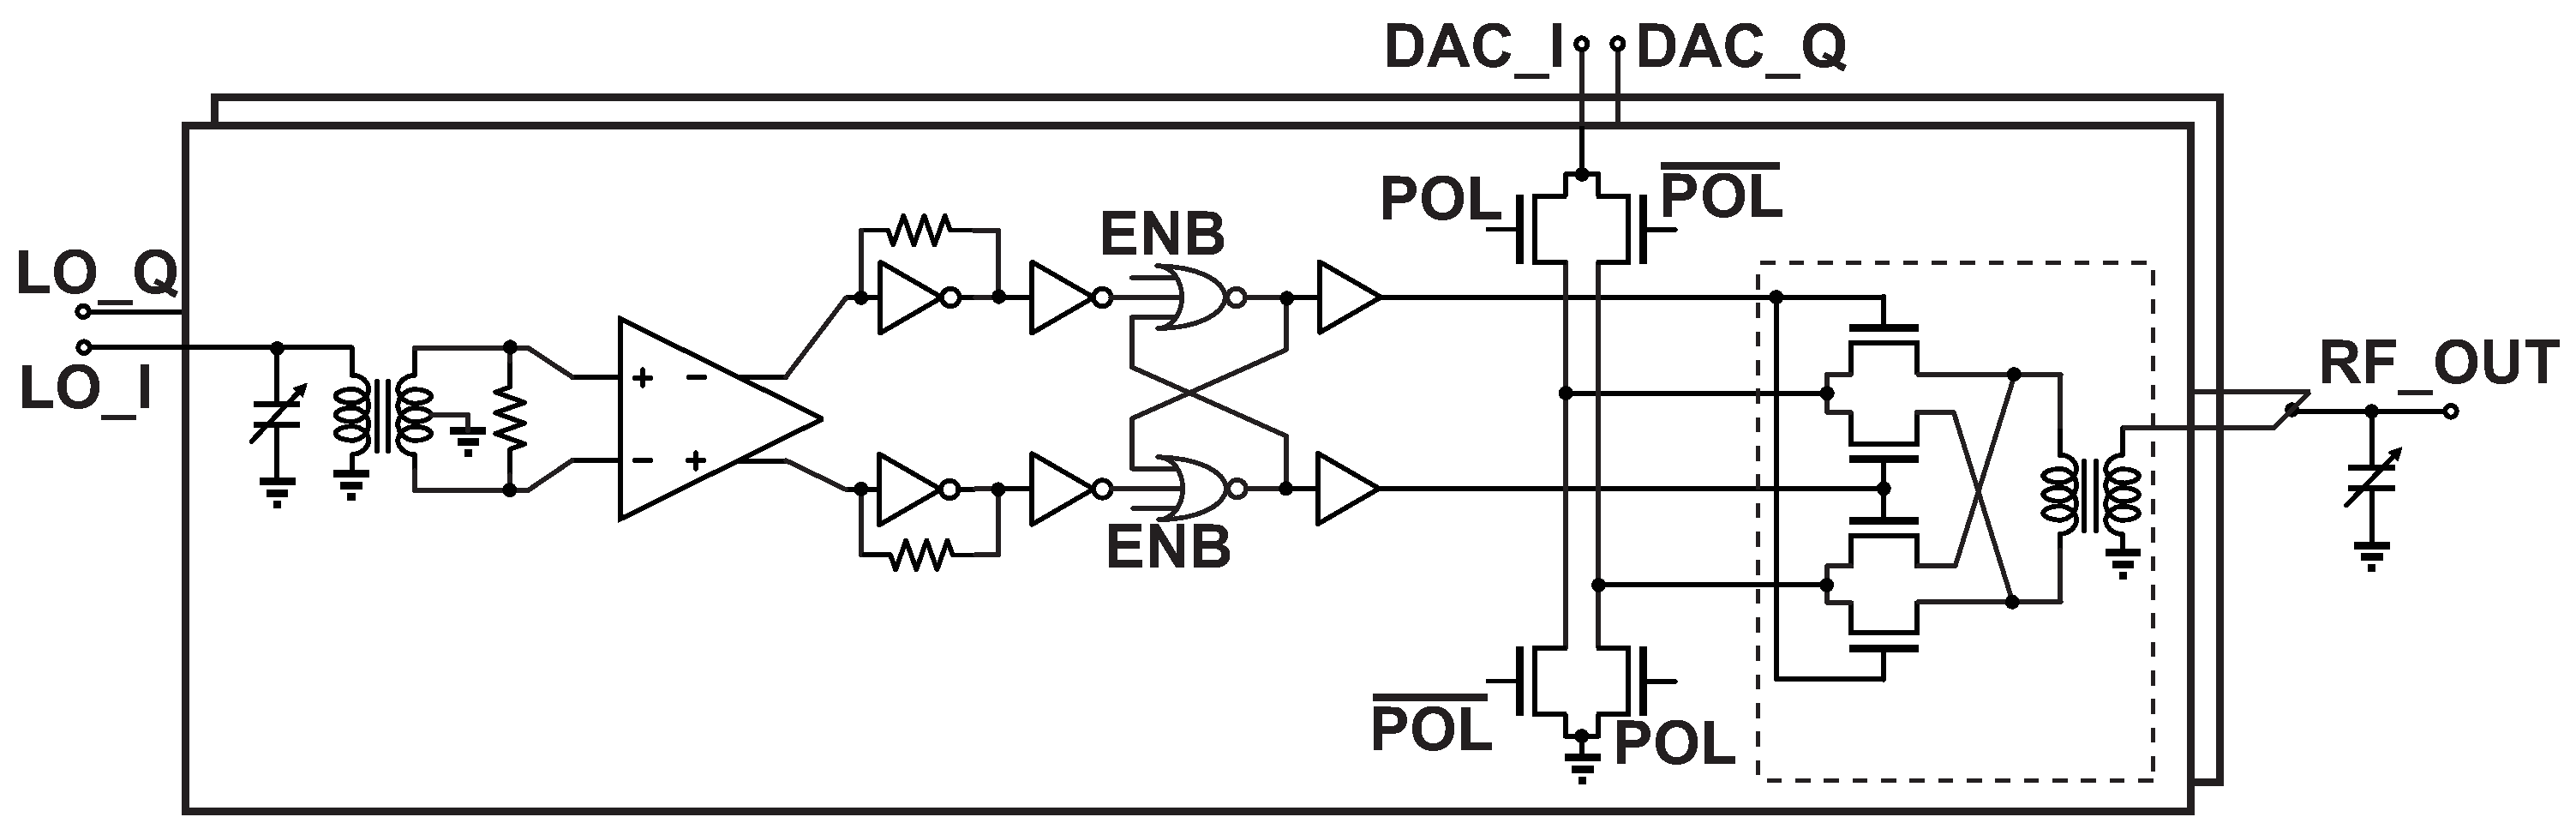
\includegraphics[width=\columnwidth]{Figures/FIGURE_10}
\caption{Schematic diagram of the vector modulator.}\label{vectormod}
\end{figure}

The IF currents from each envelope DAC are routed through one arm of a polarity switch---required to achieve a full 360$^\circ$ of carrier phase control---through the mixer, and back through the other arm of the polarity switch to ground. The \CR{RF port} of the mixer is transformer coupled to the output, where the two quadratures are combined in the voltage domain. Finally,  \CR{the output transformer network} also features a bondpad-side capacitive tuning network that can be used to optimize coupling over the full 4--8\,GHz frequency range. \CR{This network also serves as a low-Q filter, which is especially useful in rejecting odd-order harmonics of the generated pulses.}

\begin{figure*}[bt!]\begin{center}
\CR{\includegraphics[width=2\columnwidth]{Figures/FIGURE_11}}
%\subfigure[]{
%\includegraphics[height=1.77in]{Figures/Diephoto}}
%\subfigure[]{\includegraphics[height=1.77in]{Figures/Die_Mid.jpg}}
%\subfigure[]{\includegraphics[height=1.77in]{Figures/Module.jpg}}
\end{center}
\caption{(a) Die micrograph. The chip measures 1.1\,mm by 1.6\,mm. (b) Photograph of packaged integrated circuit. The chip was mounted within a pocket of a printed circuit board to minimize the RF bondwires. (c) Photograph of module used for testing.}\label{diephoto}
\end{figure*}

\begin{figure*}[bt!]\begin{center}
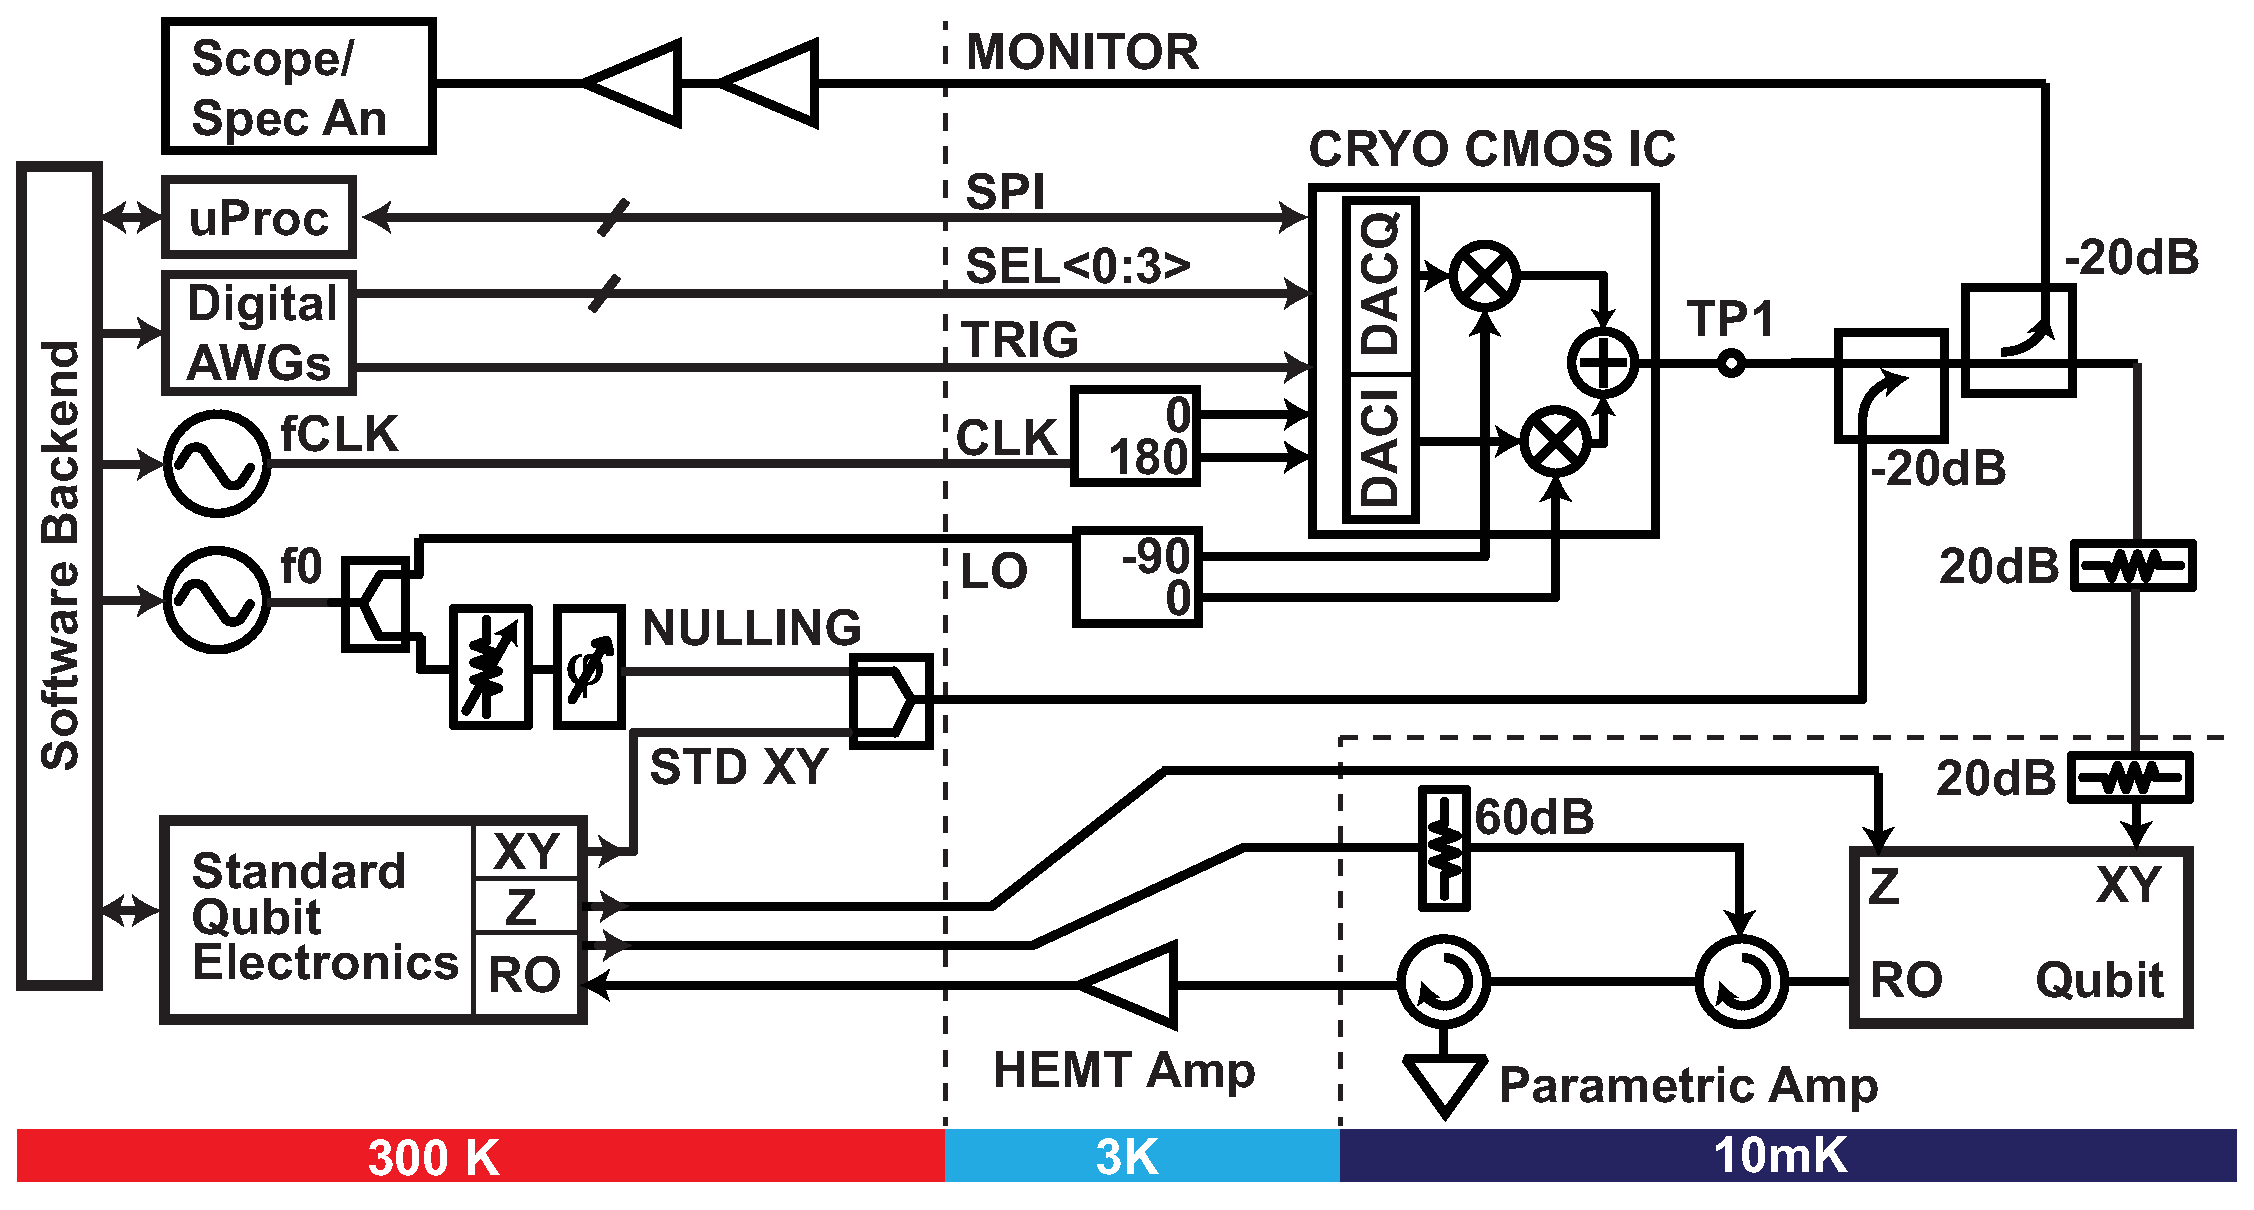
\includegraphics[width=1.5\columnwidth]{Figures/FIGURE_12}
\caption{Simplified block diagram of the test setup used for quantum control experiments.}\label{setup}\end{center}
\end{figure*}

In combination, the number of configuration bits available to tailor the shape\CR{,  amplitude, and carrier phase} of the control pulses exceeds that required to meet the amplitude and phase resolution specifications set out in Section~\ref{requirements}. However, the circuit was over-designed in order to ensure robustness against changes with cryogenic cooling. %In the future the power could be reduced by lowering the resolution.
In addition, for
simplicity, no provision was made to null LO leakage, as it can be canceled off-chip
and was not viewed as a fundamental limitation. This functionality could be
added to a future design.


\section{Results}
The pulse modulator was implemented in a 28-nm CMOS process and a die photo appears in Fig.~\ref{diephoto}(a). The chip was packaged in a module for testing. As shown in Fig.~\ref{diephoto}(b), the die was mounted within a cutout in a printed circuit board so as to minimize bondwire lengths and provide a direct thermal path from the chip to the metallic chassis. A photograph of the module appears in Fig.~\ref{diephoto}(c). %In addition to the integrated circuit, test transistors from each transistor family (e.g., uLVT, LVT, etc) were also fabricated to enable benchmarking of the technology and these devices were evaluated prior to characterization of the quantum control IC. 
%\subsection{Technology Characterization}
%Test structures from each transistor family from the 28-nm CMOS process were characterized on-wafer at both 300\,K and 7\,K. DC IV curves were acquired using a semiconductor analyzer and used to extract sub-threshold slopes, threshold voltages, extrinsic transconductances, and extrinsic output conductances for each device. The transistors were biased through a bias-tee for these measurements to permit termination of the RF port, so as to reduce the probability of oscillation. Scattering parameters were also acquired for each device as well as open/short de-embedding structures  over the frequency range of 0.01-to-67\,GHz. The resulting data were used to determine values of the unity current gain cutoff frequency ($f_\text{t}$) and the maximum frequency of oscillation ($f_\text{MAX}$) as a function of bias for each device. 

%{\color{red}In all cases, the magnitude of the threshold voltages voltages increased, with }




Prior to characterizing the IC, we first performed baseline measurements of test structures for each of the different transistor flavors that are available in the 28-nm CMOS process. These measurements were carried out to ensure that the temperature dependence of devices with different doping profiles and polarities is similar to that previously reported for a single minimum-length 28-nm NMOS device~\cite{beckers2018characterization}. Measurements were carried-out on\CR{-}wafer at 300 and 7\,K,\footnote{\CR{These measurements were made with a Lakeshore CRX-4K cryogenic probe station, which can reach 5.5\,K when the heat load is minimized. Here, we selected an ambient temperature of 7\,K to ensure the base temperature could be maintained across all measurements. It is expected that the performance at 7\,K is indicative to that at 3\,K, as the terminal characteristics change little in this range.}} and key parameters such as threshold voltage, sub-threshold \CR{swing}, extrinsic transconductance ($G_\text{m}$), and unity current gain cutoff frequency ($f_\text{t}$) were extracted and display similar trends among the different device families. On average, the threshold voltages increased by a factor of 40\% whereas the sub-threshold \CR{swing}, extrinsic transconductance, and unity current gain cutoff frequency improved by factors of 4.6, 2, and 1.8, respectively. \CR{These values are consistent with previously observed values for a variety of nanometer technologies\footnote{\CR{To the best of our knowledge, data describing the temperature dependence of $f_\text{t}$ of a nanometer-scale MOSFET biased at a fixed current are not available in the literature. However, based upon the results in~\cite{coskun2014cryogenic}, an increase in $f_\text{t}$ of approximately 75\% is expected with cryogenic cooling.}}~\cite{beckers2018characterization,IEDM_CHARBON,beckers_GM,coskun2014cryogenic}}. Here, the small-signal metrics are specified at a current density of 10\,mA/mm. It is interesting to note that \CR{most} changes \CR{were found to be} consistent for both PMOS and NMOS devices. The full set of extracted parameters is provided in Table~\ref{transistors} of the Appendix. 
%\subsection{Quantum Control Ex periments}

After evaluating the transistor performance, the low-temperature operation of the chip was evaluated through a series of quantum control experiments. To facilitate these measurements, the packaged IC was mounted on the 3-K stage of a commercial dilution refrigerator and interfaced to a qubit mounted on the 10\,mK stage of the system. The qubit employed for this experiment was a transmon that is part of a 5-qubit processor and is characterized by an anharmonicity parameter, $\eta/2\pi\approx-330\,$MHz. For all measurements, the other four qubits were tuned to be as far away in frequency as possible so as to make their presence inconsequential.

A detailed block diagram of the test setup appears in Fig.~\ref{setup}. The module containing the CMOS IC was mounted on the 3-K stage of the refrigerator, along with 90- and 180-degree hybrids, which were used to interface to the LO and clock ports of the chip, respectively. The LO and clock signals were generated at room temperature using commercial synthesizers. 

The LO signal was split at room temperature to enable feed-forward cancellation of LO leakage to the RF output port of the cryo-CMOS IC module. Vector modulation of the leakage cancellation tone was achieved using a digital step attenuator followed by a digital phase shifter. The amplitude and phase shifted cancellation signal was then combined with the RF output of the IC using a 20-dB coupler, mounted on the 3-K stage of the cryostat.  In concert with a power combiner added after the phase shifter, this coupler also provided a mechanism to inject a standard XY control signal, thereby enabling baseline measurements.

A second 20-dB coupler was employed at the 3-K stage to couple a small fraction of the RF output back to room temperature. This weak monitor signal was further amplified by approximately 50\,dB, such that it could be viewed on an oscilloscope for debugging purposes. 

Finally, the RF output was attenuated by 40\,dB and connected to the XY port of the qubit. The Z and readout terminals of the qubit were connected to standard Z and readout electronics chains to complete the analog portion of the measurement setup. 

The \CR{chip's serial programming interface (SPI)} was interfaced to a microprocessor, allowing for simple integration into a software stack. Finally, the trigger and word select lines of the CMOS IC were driven by a bank of AWGs, configured to operate with binary outputs. All instruments were under the control of a standard qubit software stack, with the necessary drivers added to control the CMOS IC within a standard experimental flow. 

Once the setup was complete, the system was cooled to base temperature. The qubit was calibrated using  standard room temperature control and readout electronics.  Next a series of experiments were employed to evaluate the performance of the IC and compare it to that of conventional room temperature control electronics, as detailed below. The CMOS IC was powered down for all baseline measurements. Unless otherwise stated,  the qubit was tuned to 5.6\,GHz for all measurements. 

\subsection{Preliminary Room Temperature Measurements}
Prior to cooling the system down, a set of measurements were carried out to ensure that the \CR{basic operation of the CMOS IC was as expected}. For these measurements, a coaxial cable was connected directly to the output of the module and the performance was monitored both on an oscilloscope and a spectrum analyzer.  %The circuit was found to be operational for clock and LO signals in the range of 0.5-to-3\,GHz and 4-to-8\,GHz, respectively. 
\CR{The circuit was found to be operational for clock frequencies up to 3\,GHz and LO frequencies from 4-to-8\,GHz.} The power required to drive the inputs of the clock and LO hybrids was less than $-20\,$dBm at 2\,GHz and $-10\,$dBm at 5.6\,GHz, respectively.  Example time-domain waveforms appear in Fig.~\ref{timedomain}. For this measurement, the waveform memory was initialized with a set of sixteen different waveforms and the select lines were used to rotate between these different instructions. \CR{The clock and carrier frequencies were set to 2.0 and 5.6\,GHz, respectively}.

\subsection{LO Leakage Cancellation} %As the integrated quantum controller employs a direct conversion architecture, any local oscillator leakage that couples to the RF output will be at the qubit drive frequency. As described in Section~\ref{ONOFF}, such leakage will both limit gate fidelity and lead to initialization errors. 
Once the \CR{dilution refrigerator} reached base temperature, we first minimized the LO leakage using the \CR{nulling} path shown in Fig.~\ref{setup}.  The qubit was first initialized to the ground state and then allowed to idle for a period, $\tau$, before its state was measured. The magnitude and phase of the cancellation tone were then varied to minimize the measured $|1\rangle$ state population.  The resolution employed for amplitude and phase control was 0.25\,dB and 1$^\circ$, respectively\footnote{It may seem like a more direct approach one could take to null the LO feed through is to look at it on a spectrum analyzer, taking advantage of the monitor port that we have built into our test setup. However, we found that this was actually an ineffective method that did not produce nominal settings. We believe this is either due to the finite directivity of the directional coupler or secondary paths through which the LO signal leaked to the spectrum analyzer.}. We found that the nominal settings depended strongly on the impedances presented by the LO and RF ports of the IC (which could be varied through the transformer tuning capacitors). However, we also determined that these values were repeatable and stable on timescales of several days. As such, it appears feasible to implement leakage nulling in a future version of the chip.

\begin{figure}[bt!]
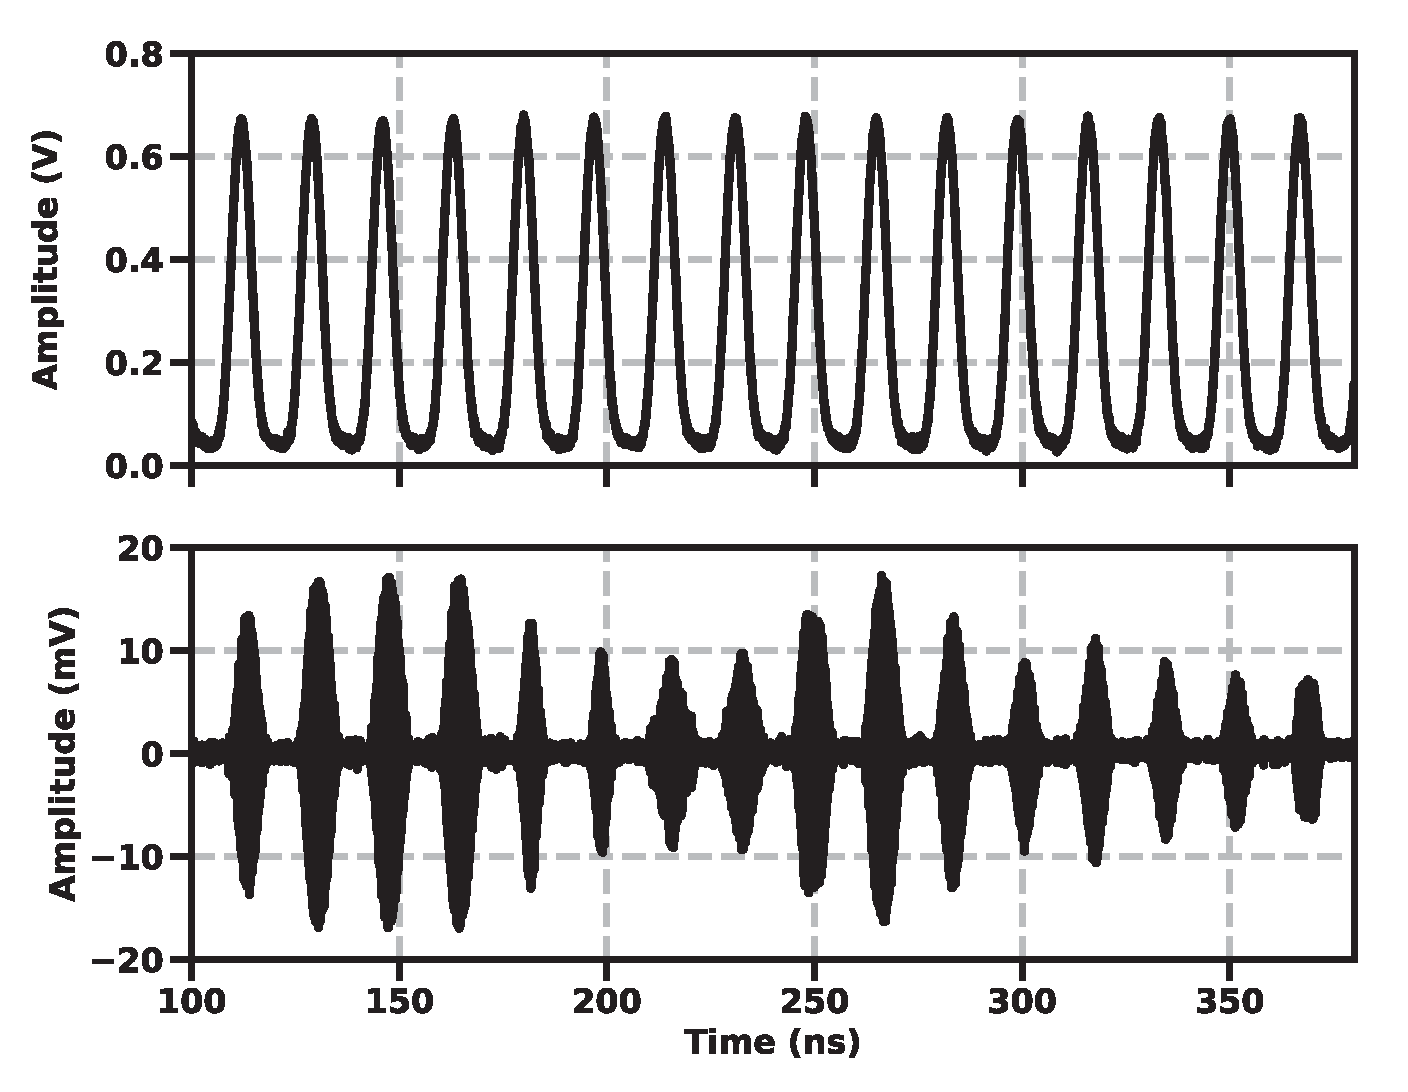
\includegraphics[width=\columnwidth]{Figures/FIGURE_13}
\caption{Example time domain trigger (top) and pulse (bottom) waveforms, measured at 300\,K. The chip was initialized with sixteen different waveforms and stepped through using the select lines. For these measuremenst, the chip was driven with a 2\,GHz sample clock. A cable loss of approximately 5~dB has not been de-embedded from the measurement results.} \label{timedomain}
\end{figure}
\begin{figure}[bt!]
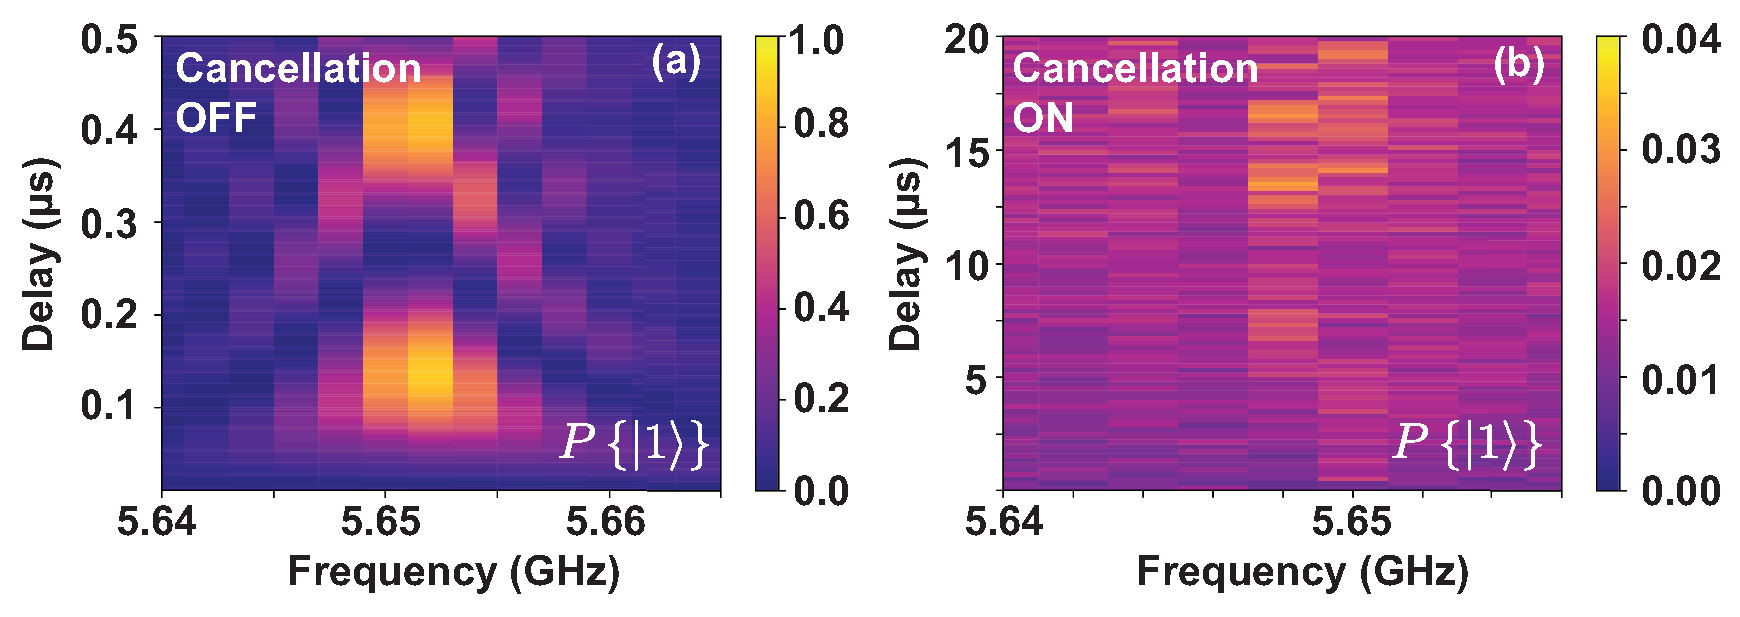
\includegraphics[width=\columnwidth]{Figures/FIGURE_14}
\caption{Effect of local oscillator feedthrough. (a) When the LO cancellation circuit is off, the qubit is driven by the LO leakage. (b) With the LO cancellation circuit on, nearly all $|1\rangle$ state population is supressed. }\label{LOONOFF}
\end{figure}
Example results in which the cancellation is turned OFF and ON are shown in Fig.~\ref{LOONOFF}. For these measurements, the qubit was tuned to 5.65\,GHz. With the cancellation disabled, Rabi oscillations were observed with a period of approximately 300\,ns. \CR{This implies a 26\,dB ON/OFF ratio, assuming raised-cosine pulses of 15\,ns in duration are employed}. \CR{This modest ON/OFF ratio is likely explained by  the  close proximity of the RF and LO wirebonds (see Fig.~\ref{diephoto}(b)) as well as finite LO-IF isolation in the mixers}. 
On the other hand, with the cancellation enabled, we found that the LO leakage was reduced to the level that a $|1\rangle$ population of less than 4\% was observed after 20\,$\mu$s of idling. This level of unintended drive is  acceptable, as it corresponds to an error of less than \CR{0.001\%} on the timescale of a gate operation. 

\subsection{Amplitude Control}(controlled by $I_\text{P}$)
Next, we preformed a Rabi oscillation experiment in order to evaluate the feasibility of deterministically inducing XY rotations using the CMOS IC. The protocol for this experiment\CR{---}described in Fig.~\ref{rabisingle}(a) and~\ref{rabisingle}(b)\CR{---}was to initialize the qubit to the $|0\rangle$ state, excite it with a raised cosine pulse of \CR{21\,ns} in duration, and then measure the qubit state. \CR{At each point, 5,000 state statistics were recorded to enable the estimation of state probabilities. For simplicity, these measurements were carried-out with only one of the two quadratures enabled.}

%The experiment was repeated for a wide range of envelope amplitudes and 5,000 statistics were taken for each setting. 

\CR{The Rabi amplitude experiment was conducted in two different manners. First, the amplitude was varied by sweeping the DAC reference current ($I_\text{N}$) through its full 8-bit range while fixing the sub-DAC settings for a maximum-amplitude raised-cosine envelope. Next, the experiment was repeated with the DAC reference current fixed in the middle of its range and a scaling factor---swept from 0-to-1---applied to all of the sub-DACs to generate a nominally raised cosine envelope of varying amplitude.  In both experiments, the full scale of the reference DAC was set to the middle of its range (by setting $I_\text{P}$ appropriately). Example Rabi oscillations for each experiment appear in Figs.~\ref{cal}(a) and \ref{cal}(b). In both cases, non-monotonicity and nonlinearity was observed, but this non-ideal behavior was found to be  much stronger when the reference DAC was used to vary the pulse amplitude.}  

%While the measured statistics would nominally be plotted against the programmed envelope amplitude setting, we found that the DACs were both non-monotonic and nonlinear when operated at cryogenic temperatures. 

\CR{To understand this behavior and create calibrated Rabi oscillation curves, we next measured the relative pulse amplitude as a function of configuration settings using a spectrum analyzer connected to the monitor port (see Fig.~\ref{setup}). Representative curves for the same conditions used to obtain Figs.~\ref{cal}(a) and \ref{cal}(b) appear in Figs.~\ref{cal}(c) and ~\ref{cal}(d), respectively. Significant non-linearity and non-monotonicity was observed when the reference DAC current was employed to vary the pulse amplitude. This behavior may be related to a combination of the sub-threshold operation of the reference DAC, the small transistor sizing, the lack of thermometer coding,  the relatively low impedance associated with the (non-cascoded) current mirror employed here, and/or leakage in the PMOS current mirror circuit. On the other hand, the measured pulse amplitude was found to be far more linear as a function of the scaled reference sub-DAC amplitudes (see Fig.~\ref{cal}(d)). This could be due to the fact that the sub-DACs were operated more into the saturation regime in comparison to the reference DAC.}

%A representative plot of the measured envelope amplitude as a function of the reference DAC setting appears in Fig.~\ref{cal}(a). For this measurement, the sub-DACs were programmed to produce a nominally raised cosine envelope and the current, $I_\text{P}$, driving the reference DAC was set towards the middle of its range. Significant non-linearity and non-monotonicity was observed. This behavior may be related to a combination of the sub-threshold operation of the reference DAC, small transistor sizing, lack of thermometer coding, and the relatively low impedance associated with the (non-cascoded) current mirror employed here.

%We also considered varying the pulse amplitude by scaling the weights of each of the eleven sub-DACs. The measured pulse amplitude is plotted as a function of relative envelope amplitude in Fig.~\ref{cal}(b). The results still display nonlinearity and non-monotonicity, but to a much lesser extent than in the case where the reference amplitude was swept. This is likely due to the fact that the sub-DACs were operated further into the saturation regime and thus were less sensitive to mismatch effects.} %As such, we made an independent measurement of the pulse amplitude as a function of digital setting by using a spectrum analyzer to measure an amplified version of the signal at the monitor port (see Fig.~\ref{setup}). %\CR{Example calibration curves appear in Fig.~\ref{xx}.}

%\CR{Figs.~\ref{cal}(c) and \ref{cal}(d) show the measured Rabi oscillations corresponding to the reference DAC and envelope amplitude sweeps described above. Each point represents the average of 5,000 measurements. The curves were found to be repeatable and agree well with expectation, based upon the curves shown in Fig.~\ref{cal}(a) and \ref{cal}(b).} 

\begin{figure}[bt!]
\includegraphics[width=\columnwidth]{Figures/FIGURE_15}
\caption{\CR{Rabi oscillation experiment protocols. (a) Experimental protocol and (b) Bloch sphere trajectory for single-pulse Rabi oscillation experiment. (c) Experimental protocol and (d) Bloch sphere trajectory for two-pulse Rabi experiment. All pulses had a duration of 21\,ns.}}\label{rabisingle}
\end{figure}

%\CR{A calibrated Rabi oscillation curve appears in Fig.~\ref{rabidual}(a). For this measurement, the envelope settings ($I_\text{1}$--$I_\text{11}$) were programmed to provide a nominally raised-cosine envelope waveform and the amplitude was varied by stepping the DAC reference current ($I_\text{N}$) through its full 8-bit range. 5,000 statistics were collected at each point and sweeps were carried out for eleven different values of the reference current supplying the amplitude DAC ($I_\text{P}$).}  
\CR{With the envelope amplitudes characterized, we next generated calibrated Rabi oscillation curves, an example of which appears in Fig.~\ref{rabidual}(a).}  The data reported on this figure were acquired by  sweeping the DAC reference current ($I_\text{N}$) through \CR{its full 8-bit range} for eleven different \CR{full-scale values, set by adjusting the reference current, $I_\text{P}$}. Data \CR{are} not shown for x-axis values below 0.22 since there was insufficient SNR to measure the envelope amplitude using the spectrum analyzer. The results in Fig.\CR{~\ref{rabidual}(a)} show the expected behavior: the maxima of the $|0\rangle$ and $|1\rangle$ state probabilities are consistent with separately measured $|0\rangle$ and $|1\rangle$ state readout error rates of 2.4\% and 6.8\%, respectively.
\begin{figure}[bt!]
\centering
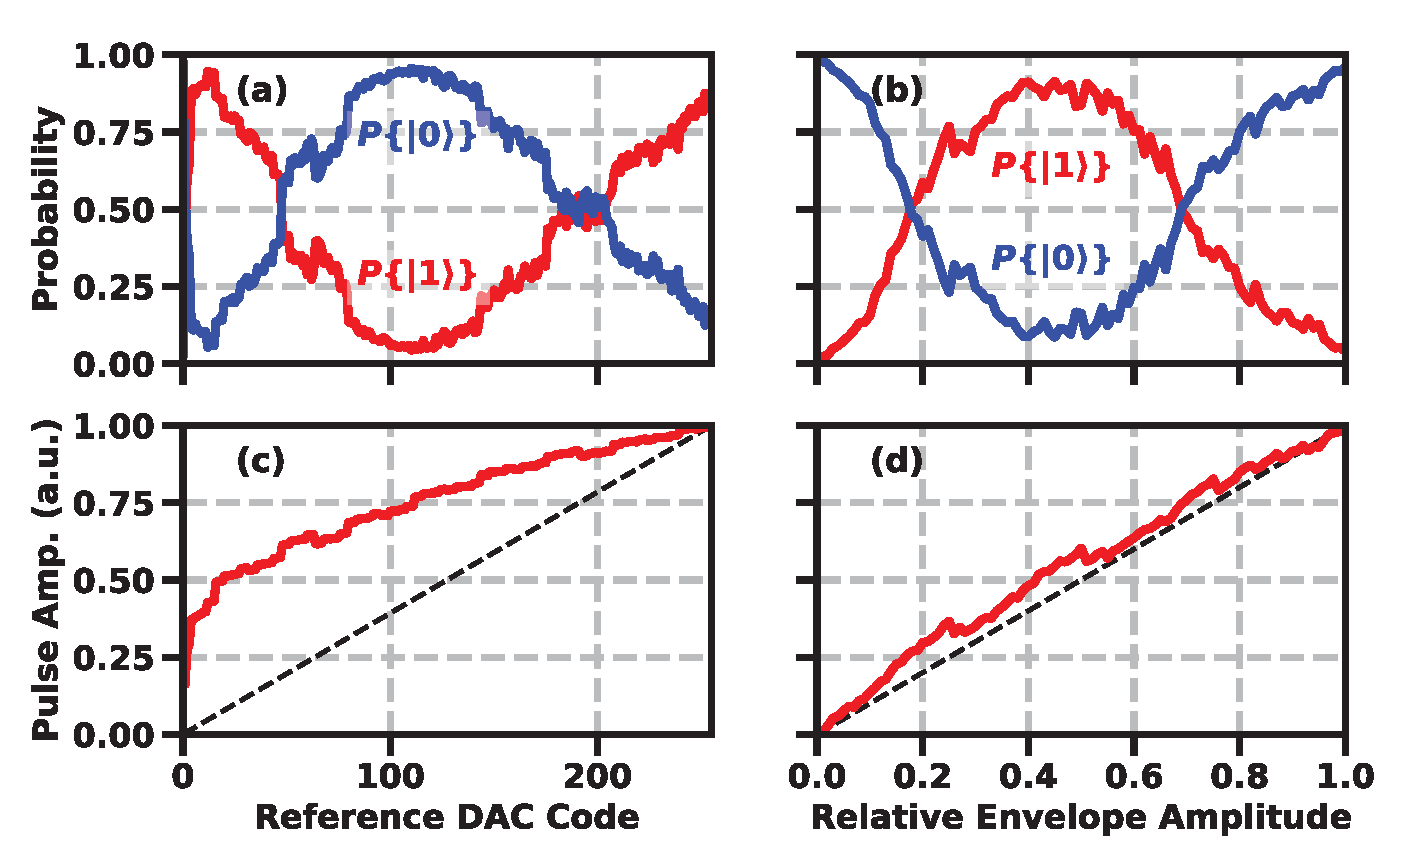
\includegraphics[width=\columnwidth]{Figures/FIGURE_16}
\caption{\CR{Uncalibrated amplitude performance of quantum controller. Examples of measured envelope amplitude as a function of (a) reference current ($I_\text{N}$) DAC setting (swept from 1-to-255) and (b) relative envelope DAC amplitude (swept by scaling the weights of each sub-DAC with a coefficient ranging from 0-to-1). Corresponding Rabi oscillations for the (c) reference current and (d) envelope amplitude sweeps. In both cases, the sweeps were carried-out with the current source supplying $I_\text{P}$ to the reference DAC set near its mid-range value. }}\label{cal}
\end{figure}
\begin{figure}[bt!]
\includegraphics[width=\columnwidth]{Figures/FIGURE_17}
\caption{\CR{Calibrated Rabi oscillation experiments for (a) single- and (b) dual-pulse excitation. High-visibility Rabi oscillations were observed in both cases and, as expected, the period for the dual-pulse experiment was approximatley half of that of the single-pulse experiment. All pulses had a duration of 21\,ns.}}\label{rabidual}
\end{figure}

A second Rabi experiment was conducted to further explore the ability to drive XY rotations. In this experiment, described in \CR{Fig.~\ref{rabisingle}(c) and \ref{rabisingle}(d)}, the same protocol was employed except the qubit was excited with an extra pulse before being measured. As such, the qubit should experience a factor of two larger rotation. As expected, the Rabi oscillations in Fig.~\ref{rabidual}\CR{(b)} display about a factor of two higher frequency of oscillation in comparison to the previous case in which the qubit was only excited by a single pulse. 


\subsection{Coherent Control and Fast Switching}
The previous experiment showed that it is possible to accurately drive rotations using the cryo CMOS IC, but it did not probe the ability to control the axis of rotation. To test the coherent control and fast-switching capabilities of the chip, a three-pulse experiment was carried out. The experimental protocol is described in Figs.~\ref{Ramsey}(a) and \ref{Ramsey}(b). The qubit was first initialized to the ground state and then excited by a series of three pulses. The first and third pulses were $X$ pulses of varying amplitude, $\theta_\text{A}$, whereas the middle pulse was a $\pi$-pulse with varying carrier phase, $\phi_\text{B}$. After the third pulse, the state of the qubit was measured. \CR{For this experiment, we fixed the I and Q channel reference DAC currents ($I_\text{N}$) and scaled the individual sub-DAC weights ($I_\text{1}$--$I_\text{11}$) proportionally to adjust the pulse amplitude and carrier phase. This approach was selected since we found that it produced less non-linearity/non-monotonicity than what was achieved when adjusting the reference current (see Fig.~\ref{cal}).} 

It can be shown that the unitary evolution \CR{resulting} from this pulse sequence ideally leaves the qubit in a state such that, if measured, the probability of being in the $|0\rangle$ state depends on both $\theta_\text{A}$ and $\phi_\text{B}$:  
\begin{figure}[bt!]
\includegraphics[width=\columnwidth]{Figures/FIGURE_18}
\caption{Three pulse experiment used to evaluate fast switching and phase coherent features of the IC. (a) Experimental protocol. (b) Example qubit trajectory for $\theta_\text{A}=\pi/2$ and $\phi_\text{B}=5\pi/9$. (c) Measured $P\left\{|0\rangle\right\}$ for standard XY control electronics. (d) Measured $P\left\{|0\rangle\right\}$ for cryo-CMOS XY controller. (e) Residual error for standard XY controller. (f) Residual error for cryo-CMOS XY controller. No calibration was performed for the envelope amplitude or carrier phase generated by the cryo-CMOS controller and it is believed that the residual could be  reduced significantly if a calibration were carried out.}
\label{Ramsey}
\end{figure}
\begin{equation}
P\left\{|0\rangle\right\}=4\cos^2\left(\phi_\text{B}\right)\sin^2\left(\frac{\theta_\text{A}}{2}\right)\cos^2\left(\frac{\theta_\text{A}}{2}\right).\label{idealram}
\end{equation}
As such, the experiment should produce a maximum probability of returning $|0\rangle$ when $\phi_\text{B}=0,\pi$ and $\theta_\text{A}=\pi/2,3\pi/2$.

The experiment was carried-out using both the standard control electronics and the CMOS IC and the results appear in Figs.~\ref{Ramsey}(c) and \ref{Ramsey}(d), respectively. In both cases, the general structure is consistent with expectation, however the CMOS IC results appear noisier than those of the standard control electronics. However, this is explained by the fact that the envelope amplitude and carrier phase generated by the CMOS IC were not calibrated in this experiment. The residual error obtained by taking the difference between the measured and ideal results (i.e., equation~(\ref{idealram})) is shown for the baseline measurement and the CMOS IC in Figs.~\ref{Ramsey}(e) and \ref{Ramsey}(f), respectively. \CR{Referring to the plot of the residual error for the CMOS IC (Fig.~\ref{Ramsey}(d)), there is clear structure. This implies that the errors are primarily related to deterministic control errors---that is, over/under rotations and carrier phase errors---rather than stochastic errors associated with noise. As such, it should be feasible to reduce these errors significantly through optimization of the settings used to generate each pulse.}
\subsection{Qubit Relaxation Time ($T_\text{1}$)}
The relaxation time, $T_\text{1}$, for the qubit was measured using the CMOS IC as well as the baseline system and the results were compared to ensure that the CMOS IC was not introducing additional noise that could drive $\omega_\text{01}$, thereby reducing $T_\text{1}$. For this experiment, the qubit was reset to the $|0\rangle$ state, excited to the $|1\rangle$ state with a $\pi$-pulse, and a state measurement was made after a delay, $\tau$. 100,000 statistics were gathered for each value of $\tau$. 

Results are plotted in Fig.~\ref{decoherence}. As expected, we observed that the qubit relaxed exponentially in both cases. The measured values of $T_\text{1}$ were 18.3\,$\mu$s and 17.8\,$\mu$s when using the standard control electronics and the cryo-CMOS IC, respectively. It is believed that these numbers are within the measurement/fitting error, and that there was no evidence of any impact on qubit relaxation due to broadband noise \CR{or residual LO leakage}. 
\begin{figure}[bt!]
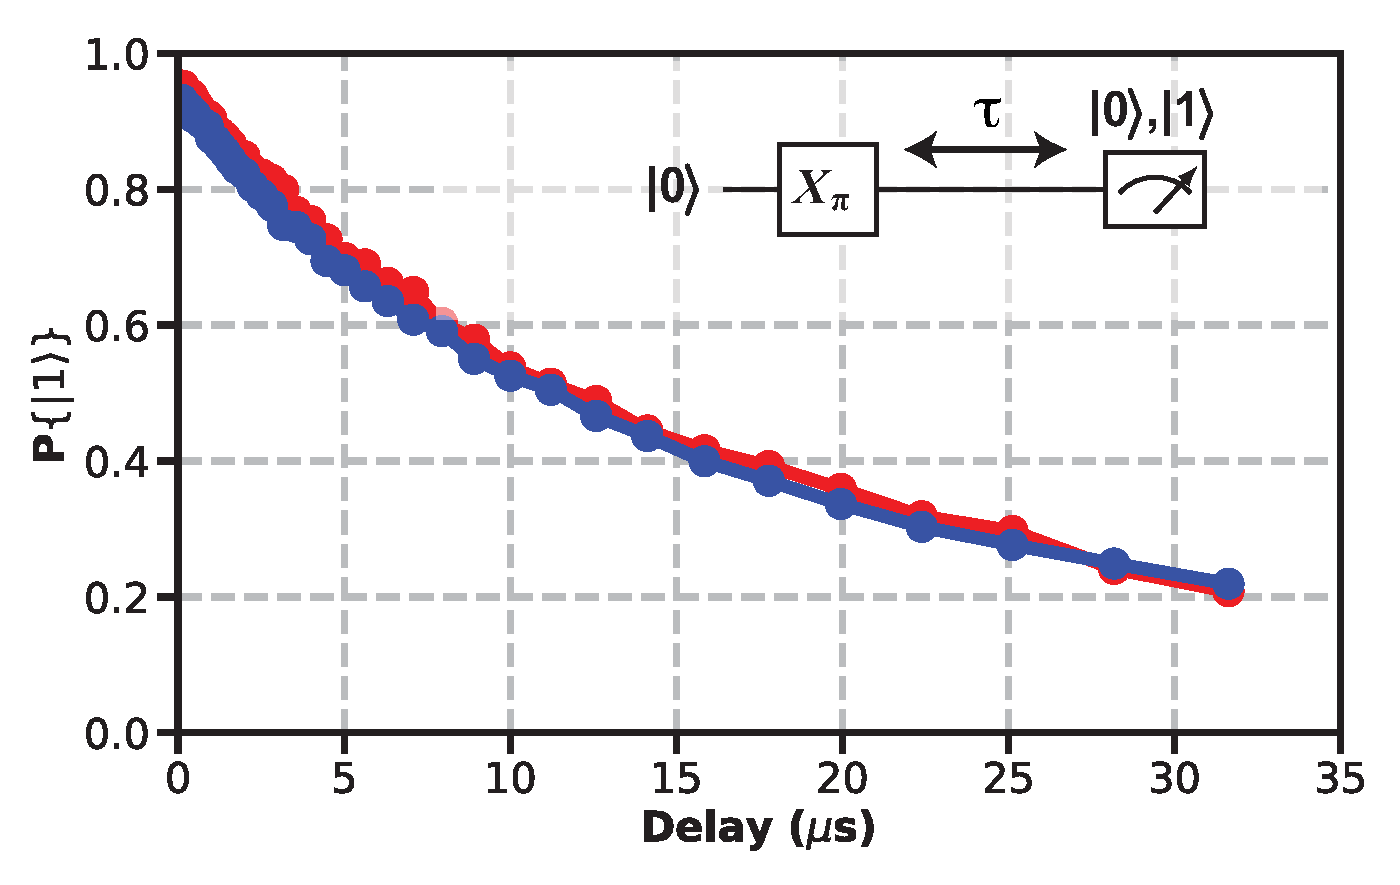
\includegraphics[width=\columnwidth]{Figures/FIGURE_19}
\caption{Qubit relaxation time measurement. The relaxation time measured using the CMOS IC (blue line) and the standard control system (dashed red line) were found to be 17.8\,\CR{$\mu$}s and 18.3\,$\mu$s, respectively. It is believed that these measurements are consistent to within the measurement repeatibility.}\label{decoherence}
\end{figure}

\subsection{Two-state population}The envelope quality (spectral width) was also evaluated. In this experiment, the qubit was first reset and then excited with a sequence of 200 $\pi$-pulses. Since any energy at the $\omega_\text{12}$ transition frequency would drive this undesired transition,  the application of 200 $\pi$-pulses should result in substantial $|2\rangle$ state population if the $\omega_{12}$ transition were even weakly excited. After the final pulse, the state was measured using a readout scheme that permitted distinguishing the $|0\rangle$, $|1\rangle$ and $|2\rangle$ states. The experiment was repeated for pulse durations ranging from 7.6--70\,ns, corresponding to clock frequencies in the range of 0.3-2.75\,GHz and 10,000 statistics were gathered at each point. A nominally raised cosine envelope shape was employed and the amplitude for a nominal $\pi$-pulse was determined independently at each clocking frequency. 

The $|2\rangle$-state measurement results appear in Fig.~\ref{twostateres} along with the measurement noise floor of 0.57\%, which was estimated from the separately measured readout infidelities. The $|2\rangle$-state population was found to be negligible for pulse durations of approximately 15\,ns or longer. However, for faster pulses, excitation of the $\omega_\text{12}$ transition was observed, with a maximum $|2\rangle$ state population \CR{at the end of the sequence} of just over 2.5\%  for a pulse duration of 7.6\,ns. The behavior is consistent with expectation, given the relatively large anharmonicity of the qubit, and would be worse for a qubit with smaller anharmonicity. 
\begin{figure}[bt!]
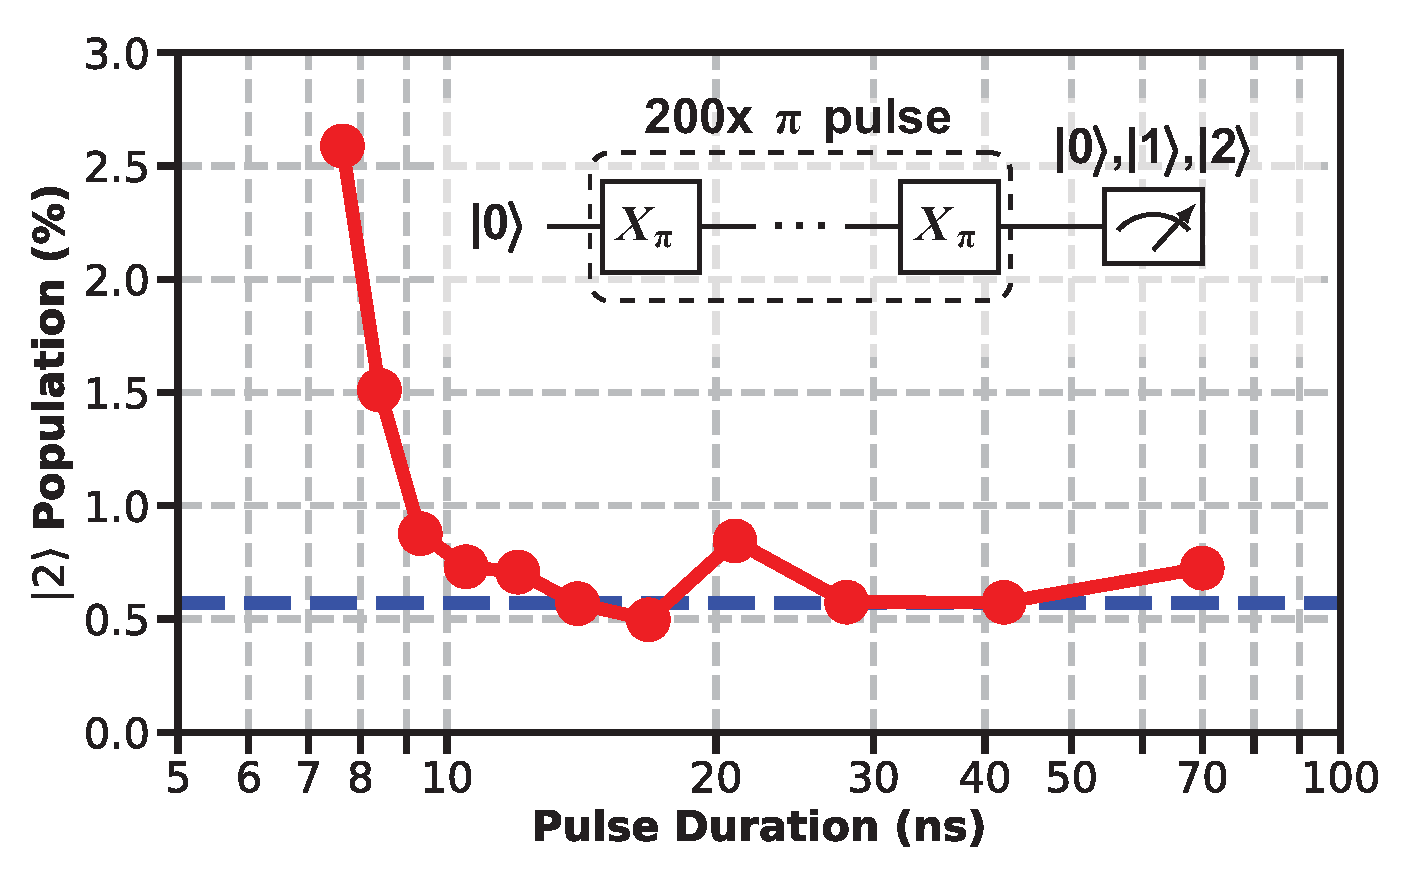
\includegraphics[width=\columnwidth]{Figures/FIGURE_20}
\caption{Two-state population as a function of pulse duration (solid red line) and two-state measurement noise floor (dashed blue line). Negligible $|2\rangle$ population was observed for gate times as short as 15\,ns.}\label{twostateres}
\end{figure}

\subsection{Comparison with state of the art}
The integrated circuit is compared with a state-of-the-art quantum control system in Table~\ref{comptab}. The measured performance is competitive with that of the standard electronics \CR{over the range of quantum control experiments which have been carried out}. However, the size, digital data-rate, and power consumption required to operate the chip are all at least an order of magnitude lower than the standard \CR{control} electronics. Of particular importance is the total power consumption, which is below 2\,mW. This number is equal to the total AC \CR{(clock and LO)} and DC power that must be delivered to the chip to drive a continuous stream of $\pi$-pulses when clocked at 1\,GHz. It is viewed to be a conservative value as the chip is expected to operate at a lower activity factor in practice. 
\begin{table}[bt!]
\caption{Comparison of CMOS IC @$f_\text{CLK}=1\,$GHz to State-of-the-art quantum control system }
\label{comptab}
\centering
\begin{tabular}{lrr}
\toprule
&Conventional Control&Cryo-CMOS IC\\
\midrule
Form Factor&Rack Mount&Integrated Circuit\\
\CR{Ambient} Temp&300\,K&3\,K\\
Update Rate&1\,GS/s&1\,GS/s\\
Instruction Set Size&N/A&16 (4-bit)\\
Digital Data Rate&28\,Gb/s&$<$0.5\,Gb/s\\
Measured $T_\text{1}$&18.3\,$\mu$s&17.8$\,\mu$s\\
$|2\rangle$ population&Negligible&Negligible\\
$\pi$-Rabi $P\left\{|1\rangle\right\}$&$\approx$95\,\%&$\approx$95\,\%\\
3 Gate RMS Error&2.5\%&11.7\%\\
Total AC+DC Power&$>1$\,W&$<2$\,mW\\
\bottomrule
\end{tabular}
\end{table}

\begin{table*}[bt!]\begin{center}
\caption{Extracted transistor parameters}\label{transistors}
\begin{tabular}{lrrrrrrrrrrrrrrrrr}
\toprule
&Temp.&uLVTn&LVTn&RVTn&HVTn&uLVTp&LVTp&RVTp&HVTp\\
\midrule
$V_\text{T}$&300\,K&0.18\,V&0.22\,V&0.26\,V&0.34\,V&0.21\,V&0.24\,V&0.29\,V&0.37\,V\\
&7\,K&0.26\,V&0.30\,V&0.35\,V&0.45\,V&0.34\,V&0.37\,V&0.40\,V&0.45\,V\\
\midrule
Sub-threshold&300\,K&\CR{100}\,mV/dec&\CR{92}\,mV/dec&\CR{84}\,mV/dec&\CR{80}\,mV/dec&\CR{103}\,mV/dec&\CR{96}\,mV/dec&\CR{87}\,mV/dec&\CR{83}\,mV/dec\\
\CR{Swing} &7\,K&\CR{16}\,mV/dec&\CR{15}\,mV/dec&\CR{15}\,mV/dec&\CR{13}\,mV/dec&\CR{33}\,mV/dec&\CR{31}\,mV/dec&\CR{30}\,mV/dec&\CR{22}\,mV/dec\\
\midrule
$G_\text{m,pk}$&300\,K&1.5\,S/mm&1.4\,S/mm&1.3\,S/mm&1.2\,S/mm&1.3\,S/mm&1.3\,S/mm&1.2\,S/mm&1.1\,S/mm\\
&7\,K&2.0\,S/mm&2.0\,S/mm&1.8\,S/mm&1.7\,S/mm&1.8\,S/mm&1.7\,S/mm&1.7\,S/mm&1.5\,S/mm\\
\midrule

$G_\text{m}$&300\,K&14\,mS/mm&15\,mS/mm&16\,mS/mm&16\,mS/mm&13\,mS/mm&14\,mS/mm&15\,mS/mm&17\,mS/mm\\
$J_\text{D}=10$\,mA/mm&7\,K&33\,mS/mm&32\,mS/mm&32\,mS/mm&31\,mS/mm&23\,mS/mm&27\,mS/mm&30\,mS/mm&28\,mS/mm\\
\midrule
$f_\text{t,pk}$&300\,K&285\,GHz&283\,GHz&284\,GHz&237\,GHz&244\,GHz&234\,GHz&230\,GHz&215\,GHz\\
&7\,K&360\,GHz&365\,GHz&347\,GHz&313\,GHz&349\,GHz&335\,GHz&327\,GHz&291\,GHz\\
\midrule
$f_\text{t}$&300\,K&52\,GHz&53\,GHz&46\,GHz&53\,GHz&49\,GHz&49\,GHz&49\,GHz&49\,GHz\\
$J_\text{D}=10$\,mA/mm&7\,K&92\,GHz&93\,GHz&89\,GHz&86\,GHz&93\,GHz&94\,GHz&89\,GHz&85\,GHz\\
%\midrule
%$f_\text{max,pk}$&300\,K&129\,GHz&126\,GHz&126\,GHz&128\,GHz&99\,GHz&98\,GHz&97\,GHz&91\,GHz%\\
%&7\,K&151\,GHz&150\,GHz&150\,GHz&145\,GHz&112\,GHz&111\,GHz&109\,GHz&111\,GHz\\
%\midrule
%$f_\text{max}$&300\,K&58\,GHz&57\,GHz&57\,GHz&67\,GHz&47\,GHz&47\,GHz&42\,GHz&41\,GHz%\\%
%$J_\text{D}=10$\,mA/mm&7\,K&80\,GHz&79\,GHz&80\,GHz&79\,GHz&59\,GHz&60\,GHz&59\,GHz&62\,GHz\\
%\midrule
%~&$T_\text{a}$ &$G_\text{m}$&$G_\text{m}$&$f_\text{t}$&$f_\text{t}$&$f_\text{MAX}$\\
%Notes&K&0.1mA/mm&peak\\
%\midrule
%uLVT&300\\
%uLVT&7\\
%\midrule
%LVT&300\\
%LVT&7\\
%\midrule
%RVT&300\\
%RVT&7\\
%\midrule
%HVT&300\\
%HVT&7\\
\bottomrule
\end{tabular}
\end{center}
\end{table*}
\section{Conclusion}
Future quantum computers will require low-power cryogenic control and readout electronics. Here, we have demonstrated a first generation quantum controller that dissipates under 2\,mW while providing \CR{promising} performance. While this is an important step towards the implementation of a scalable quantum control and measurement system, considerable research is required before such a system can be realized. 

\CR{Achieving fault tolerance will require gate error rates on the order of 0.01\% and, while we have carried out a number of quantum control experiments, we have not yet demonstrated that our prototype quantum controller contributes sufficiently low error rates to enable this level of performance. As such, an important area of future work is to establish error rates for gates carried out using the CMOS IC. Nominally, this would be done using interleaved randomized benchmarking~\cite{magesan2012efficient}, a technique used to determine the errors associated with a specific gate that is interleaved within a long sequence of gates. In this case the other gates would be generated by the standard qubit control electronics. While we do not know of any fundamental reasons that this should not be possible, there are practical challenges such as carrier phase synchronization that are currently being worked out.}

\CR{Once the performance is benchmarked, it is important to iterate on the design to improve the achievable fidelity and/or to further reduce power consumption. Example modes to improve performance include the use of improved current mirror structures and modifications to the architecture to enable DRAG and AC Stark-shift compensation. The power consumption could be reduced in a number of ways. For instance, by constraining the carrier frequency more tightly, it should be feasible to remove the LO amplification chains---which, based on room temperature simulation dissipate on the order of 250\,$\mu$W each---by reactively tuning the LO port to the mixers.}

\CR{Finally, in order for the device to truly be scalable, it must not only be power efficient, but also should require a minimum number of interconnects to room temperature. Currently, the trigger and select lines constitute a significant wiring overhead. The addition of an on-chip pulse sequencer would remove the need for these extra lines and could greatly reduce this overhead. Of course, this sequencer would ultimately need to be flexible enough to interface to a controller that selects the pulse sequences, and research is required to optimize this whole system. Finally, since transmon qubits can be made frequency tunable, it may be feasible to operate a large number of qubits with a limited number of carriers; this would greatly ease the scaling of RF lines down in to the cryogenic system by allowing reuse of LO signals. In summary, the demonstration of cryogenic control of a superconducting qubit using a cryogenic CMOS IC is an important step towards fault tolerant quantum computing, but signficant research is still  required before such a system will be feasible.}
\section*{Appendix}\
Extracted parameters for each of the transistors appear for reference in Table~\ref{transistors}.


\bibliographystyle{IEEEtran}

\bibliography{JSSC.bib}

\begin{IEEEbiography}[{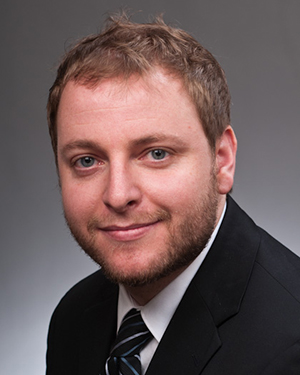
\includegraphics[width=1in,height
=1.25in,clip,keepaspectratio]{Photos_For_JSSC/BARDIN}}]{Joseph C. Bardin}
(S’01–M’10–SM’18) received the B.S. degree in electrical engineering from the University of California at Santa Barbara in 2003, the M.S. degree in electrical engineering from the University of California at Los Angeles in 2005, and the Ph.D. degree in electrical engineering from the California Institute of Technology in 2009. 

From 2003 to 2005, he was with the Jet Propulsion Laboratory, California Institute of Technology, where he was involved in the demonstration of an array-based downlink for the NASA deep-space network. From 2009 to 2010, he was a Post-Doctoral Researcher with the Caltech High-Speed Integrated Circuits Group, where he was involved in self-healing microwave receivers. In 2010, he joined the University of Massachusetts Amherst, where he is currently an Associate Professor of Electrical and Computer Engineering. Since 2017, he has also been with the Google AI Quantum, where he focuses on the development of novel integrated electronics for quantum computing. 

Dr. Bardin was a recipient of the 2011 DARPA Young Faculty Award, the 2014 NSF CAREER Award, the 2015 ONR YIP Award, the 2016 UMass College of Engineering Outstanding Junior Faculty Award, and the 2016 UMass Convocation Award for Excellence in Research and Creative Activities.
\end{IEEEbiography}

\begin{IEEEbiography}[{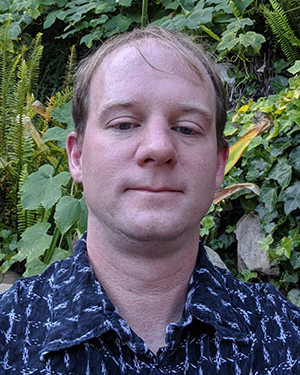
\includegraphics[width=1in,height
=1.25in,clip,keepaspectratio]{Photos_For_JSSC/EVAN}}]
{Evan Jeffrey}  received the B.A degree in physics from Washington University in St. Louis in 1999 and the Ph.D. in Physics from the University of Illinois at Urbana-Champaign in 2007.

From 2007 to 2012, he was at the University of Leiden in the Netherlands where he was involved with opto-mechanical devices in the quantum regime.  From 2012 to 2014, he was a Post-Doctoral Researcher at the University of California Santa Barbara where he was involved with superconducting qubits.  In 2014 he joined Google in Santa Barbara where he continues research on superconducting qubits.
\end{IEEEbiography}
\begin{IEEEbiography}[{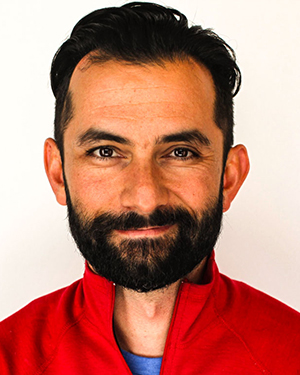
\includegraphics[width=1in,height
=1.25in,clip,keepaspectratio]{Photos_For_JSSC/ErikLucero}}]{Erik Lucero}
(S’00, M’18) received the B.S. (Hons.) degree in electrical engineering and B.S. (Hons.) degree in Applied Physics from the University of Colorado at Denver in 2005, M.A. degree in physics from the University of California at Santa Barbara in 2008, and the Ph.D. degree in physics from the University of California at Santa Barbara in 2012.

From 2001 to 2005 he was a PREP Fellow at the National Institute of Standards and Technology in Boulder, Colorado where he worked on superconducting quantum interference device arrays for the cryogenic dark matter search and a novel SQUID operational amplifier in collaboration with Professor Martin Huber at NIST and the SQUID Laboratory at the University of Colorado at Denver. In 2005 he joined Professor John Martinis’ group at the University of California at Santa Barbara, among Professor John Martinis’s first cohort of graduate students developing superconducting qubits. From 2012 to 2013, he was a Post-Doctoral Researcher at IBM T.J. Watson Research Center in Yorktown Heights, NY, where he worked on superconducting qubits. From 2013 to 2015 he worked at HRL Laboratories in Malibu, CA as a Senior Research Staff Member where he focused on quantum dots and semiconductor qubits. In 2015 he joined Google in Santa Barbara, CA. He is currently a Staff Research Scientist and the Technical Site Lead in Santa Barbara, leading production quantum hardware.
\end{IEEEbiography}

\begin{IEEEbiography}[{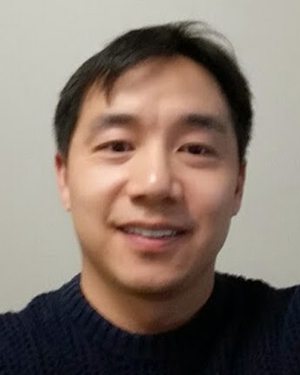
\includegraphics[width=1in,height
=1.25in,clip,keepaspectratio]{Photos_For_JSSC/TrentHuang}}]{Trent Huang} holds a Ph.D. in Electrical Engineering from Cornell University. He joined Google in 2014 as a MEMS technologist and transferred to AI Quantum Lab in 2016. 



\end{IEEEbiography}

\begin{IEEEbiography}[{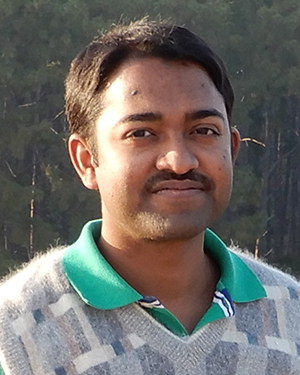
\includegraphics[width=1in,height
=1.25in,clip,keepaspectratio]{Photos_For_JSSC/sayan}}]{Sayan Das} (S'18) received the B.E. degree in electronics and telecommunication engineering from Jadavpur University, Kolkata, West Bengal, India, in 2010, the M.Tech degree in electrical engineering from the Indian Institute of Technology (IIT) Kanpur, Kanpur, Uttar Pradesh, India, in 2012, and is currently working toward the Ph.D. degree in electrical engineering at the University of Massachusetts at Amherst, Amherst, MA, USA. 

From 2012 to 2016, he was a Design Engineer at BitMapper Integration Technologies Pvt. Ltd., India where he was involved in designing and testing of electronics hardware for RF and analog systems. His current research interests include MOSFET modelling at cryogenic temperature and exploring noise and power limit of CMOS.


\end{IEEEbiography}

\begin{IEEEbiography}[{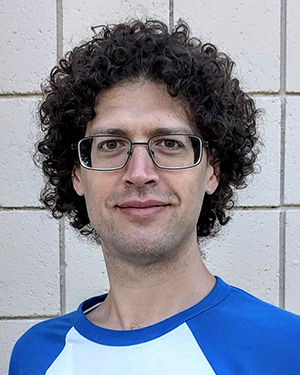
\includegraphics[width=1in,height
=1.25in,clip,keepaspectratio]{Photos_For_JSSC/Daniel}}]{Daniel Thomas Sank} was born and raised in Rockville, Maryland where he attended Wootton public high school. He earned a B.S. in physics at Yale University from 2003 to 2007, and a PhD in physics at University of California Santa Barbara from 2007 to 2014 where he worked on magnetic noise in superconducting devices and fast readout of superconducting qubits.

Since 2014, he has been a Research Scientist at Google Santa Barbara where he works on readout of superconducting qubits. His primary interests are superconducting qubit readout, electronics, and device theory.


\end{IEEEbiography}

\begin{IEEEbiography}[{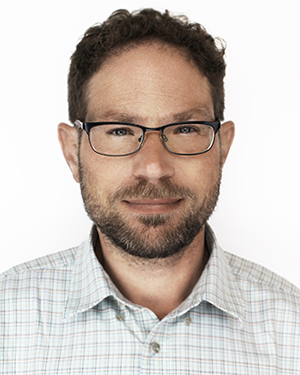
\includegraphics[width=1in,height
=1.25in,clip,keepaspectratio]{Photos_For_JSSC/ofer}}]{Ofer Naaman} received a B.Sc. degree in physics from Tel Aviv University in 1998, and a Ph.D. degree in physics from University of California, San Diego in 2003. 

From 2003 to 2007, he was a Post-Doctoral Researcher with the National Institute of Standards and Technology, where he worked on superconducting single-electron transistors. From 2007 to 2009 he was a Research Associate at the University of California, Berkeley, where he worked on quantum information in superconducting qubits and parametric amplifiers. From 2009 to 2018 he was a Physicist with Northrop Grumman Mission Systems, working on quantum information, cryogenic memory, and superconducting digital and microwave circuits. In 2018 he joined Google where he is currently a Staff Research Scientist.
\end{IEEEbiography}\vfill
\begin{IEEEbiography}[{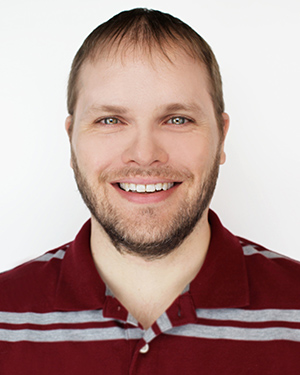
\includegraphics[width=1in,height
=1.25in,clip,keepaspectratio]{Photos_For_JSSC/AnthonyMegrant}}]{Anthony Edward Megrant} received his B.S. degree (2009) in applied physics from Cornell and Ph.D. degree (2016) in materials from University of California Santa Barbara.  

He left the US Army with an honorable discharge in 2001 as a Sergeant.  In 2015, he joined the Google AI Quantum team, where he works as a Research Scientist. 
\end{IEEEbiography}\vfill
\begin{IEEEbiographynophoto}{Rami Barends} holds a PhD in physics from Delft University of Technology, and joined Google in 2014.\end{IEEEbiographynophoto}\vfill
\begin{IEEEbiography}[{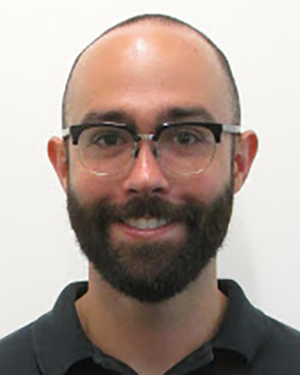
\includegraphics[width=1in,height
=1.25in,clip,keepaspectratio]{Photos_For_JSSC/Ted}}]{Ted White} received a B.S. in physics from State University of New York at Binghamton in 2009.  He then began graduate research under John Martinis and received a Ph.D. in physics from UC Santa Barbara in 2015.  

In 2015, he joined Google AI Quantum, where he is currently a senior research scientist working on superconducting quantum computing .
\end{IEEEbiography}\vfill
\begin{IEEEbiography}[{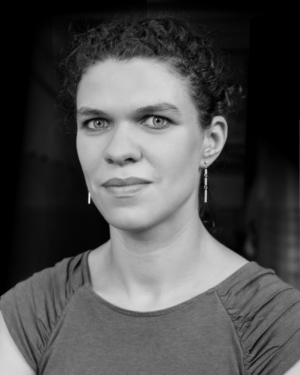
\includegraphics[width=1in,height
=1.25in,clip,keepaspectratio]{Photos_For_JSSC/mgiustina}}]{Marissa Giustina} Marissa Giustina (S’10) received the B.S. degree in mathematics from Mary Baldwin College in 2008. In 2009 and 2010 she received B.E. and M.S. degrees in engineering sciences from Thayer School of Engineering at Dartmouth College. In 2017 she received the Ph.D. degree in experimental quantum physics from Universität Wien in Vienna, Austria.

Since 2016, she has been with the Google AI Quantum research lab in Santa Barbara, CA, where she is currently a Senior Research Scientist and Quantum Electronics Engineer.


\end{IEEEbiography}
\begin{IEEEbiography}[{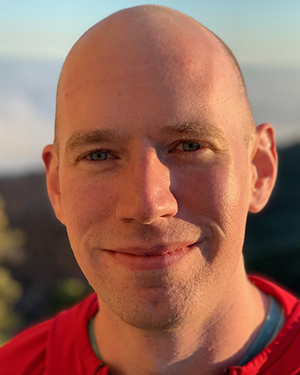
\includegraphics[width=1in,height
=1.25in,clip,keepaspectratio]{Photos_For_JSSC/kevinjsatzinger}}]{Kevin J. Satzinger}received a B.S. (2012) in physics and mathematics from Truman State University and a Ph.D. (2018) in physics from the University of California, Santa Barbara, studying the control of surface acoustic wave phonons with superconducting qubits. 

He joined Google AI Quantum as a research scientist in 2018, where he currently focuses on calibration of multi-qubit systems and entangling gates.


\end{IEEEbiography}
\begin{IEEEbiography}[{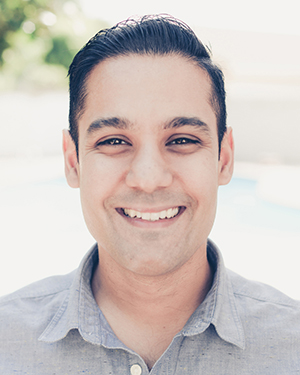
\includegraphics[width=1in,height
=1.25in,clip,keepaspectratio]{Photos_For_JSSC/KunalArya}}]{Kunal Arya} holds a M.S./PhD in Computer Engineering from the University of California, Santa Barbara and B.S. in Computer Engineering from the University of California, Santa Cruz. 

He joined Google in 2016 as a software engineer, where he works on software control infrastructure for qubit experiments.


\end{IEEEbiography}
\begin{IEEEbiography}[{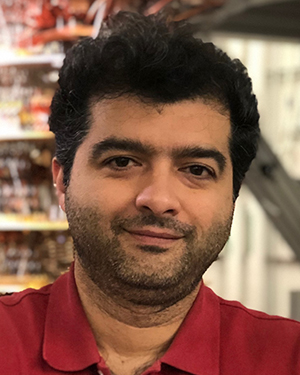
\includegraphics[width=1in,height
=1.25in,clip,keepaspectratio]{Photos_For_JSSC/pedram}}]{Pedram Roushan} received the PhD in Physics from Princeton University in 2011. 

He joined the Quantum Computing group of John Martinis as a post-doc in 2011 and was one of the original members of the quantum hardware group to move to Google in 2014. He is currently a staff research scientist at Google, focusing on quantum computing technology.
\end{IEEEbiography}
\begin{IEEEbiography}[{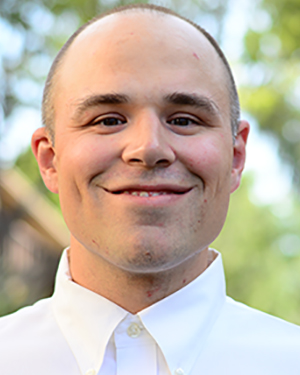
\includegraphics[width=1in,height
=1.25in,clip,keepaspectratio]{Photos_For_JSSC/Ben_Chiaro}}]{Benjamin Chiaro} holds a B.S. in Physics from the University of Wisconsin, Madison (2006) and an M.S. from the University of California, Santa Barbara (2014) .  He is currently a PhD student with the Martinis group completing his thesis research on analog control of multi-qubit systems and quantum simulation.

\end{IEEEbiography}
\begin{IEEEbiography}[{
\includegraphics[width=1in,height
=1.25in,clip,keepaspectratio]{Photos_For_JSSC/juliankelly}}]{Julian Kelly} ulian Kelly received his B.S. (2010) and PhD (2015) in physics from the University of California, Santa Barbara where he developed superconducting qubits technology in the group of John Martinis. 

In 2015, he joined the Google AI Quantum team, where he currently works as a Research Scientist. 


\end{IEEEbiography}
\begin{IEEEbiography}[{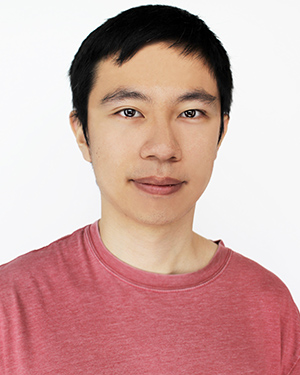
\includegraphics[width=1in,height
=1.25in,clip,keepaspectratio]{Photos_For_JSSC/zijunchen}}]{Zijun (Jimmy) Chen} received his BS in physics and mathematics from the University of Minnesota in 2008, and PhD in physics from University of California - Santa Barbara in 2018. He joined Google AI Quantum Lab in 2017, where he has been working as a research scientist.


\end{IEEEbiography}
\begin{IEEEbiography}[{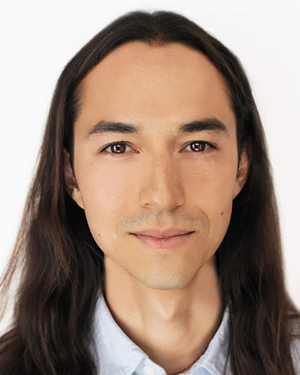
\includegraphics[width=1in,height
=1.25in,clip,keepaspectratio]{Photos_For_JSSC/BrianBurkett}}]{Brian Burkett} received his BS in physics from the University of California, Santa Barbara.  

In 2015, he joined the Google AI Quantum team as a hardware engineer, where he currently workis on developing microfabrication technologies for superconducting quantum devices.


\end{IEEEbiography}
\begin{IEEEbiography}[{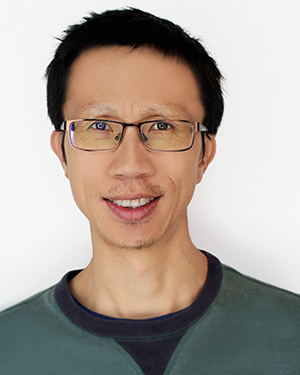
\includegraphics[width=1in,height
=1.25in,clip,keepaspectratio]{Photos_For_JSSC/YuChen}}]{Yu Chen} received a PhD in physics from University of Minnesota in 2009 and did his postdoc at the University of California - Santa Barbara from 2010 to 2014. 

He joined Google AI Quantum Lab in 2014, where he has been working as a research scientist ever since.

\end{IEEEbiography}
\begin{IEEEbiography}[{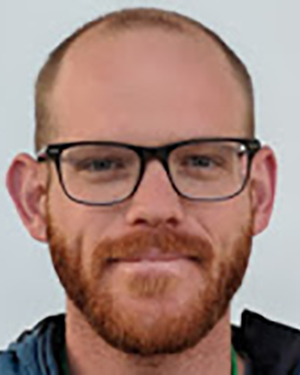
\includegraphics[width=1in,height
=1.25in,clip,keepaspectratio]{Photos_For_JSSC/Andrew}}]{Andrew Dunsworth} received a PhD in physics from University of California, Santa Barbara in 2018. In 2018, he joined Google AI Quantum Lab as a research scientist.


\end{IEEEbiography}
\begin{IEEEbiography}[{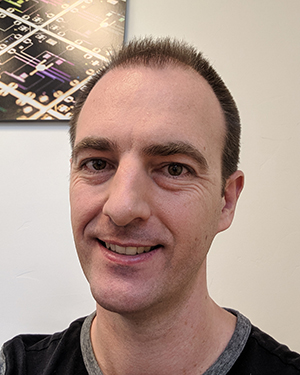
\includegraphics[width=1in,height
=1.25in,clip,keepaspectratio]{Photos_For_JSSC/AustinFowler}}]{Austin Fowler} received a PhD in Physics from the University of Melbourne in 2005 specializing in quantum computing and leaning towards quantum error correction, the focus of most of his subsequent work to date. He joined Google in 2014.


\end{IEEEbiography}
\begin{IEEEbiography}[{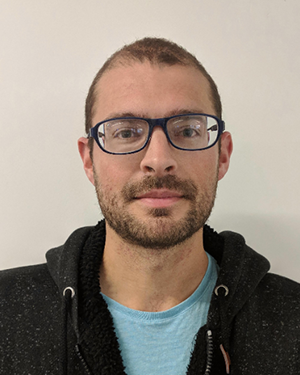
\includegraphics[width=1in,height
=1.25in,clip,keepaspectratio]{Photos_For_JSSC/BrooksFoxen}}]{Brooks Foxen} received a B.S. in physics from the University of Texas at Austin in 2007.  He then worked at National Instruments supporting conditioned measurement hardware until 2011.  In 2012 he began graduate research at the University of California at Santa Barbara under John Martinis focusing of flux control for superconducting qubits.  


\end{IEEEbiography}
\begin{IEEEbiography}[{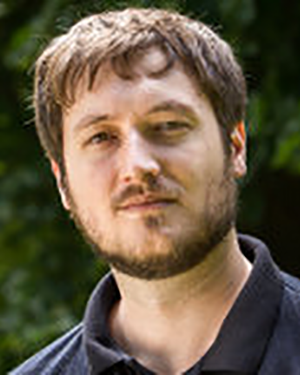
\includegraphics[width=1in,height
=1.25in,clip,keepaspectratio]{Photos_For_JSSC/craiggidney}}]{Craig Gidney} received a masters in computer science from Dalhousie University in Canada in 2013.

In 2014, he joined Google and transferred to the quantum computing 
team in 2017, where he currently serves as a quantum software engineer.


\end{IEEEbiography}
\begin{IEEEbiography}[{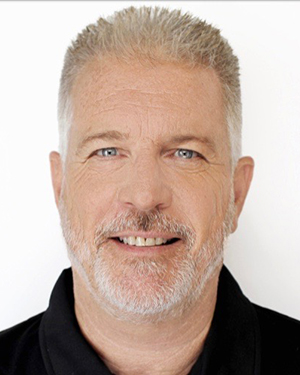
\includegraphics[width=1in,height
=1.25in,clip,keepaspectratio]{Photos_For_JSSC/RobGraff}}]{Rob Graff} is a 30 year veteran of the semiconductor industry as both an Equipment and Facilities Engineer specialising in Tech company "Start-Ups".   Since 2015, he has been working with the Google Quantum Hardware Team focusing his efforts on equipment installation and facility expansion.


\end{IEEEbiography}
\begin{IEEEbiography}[{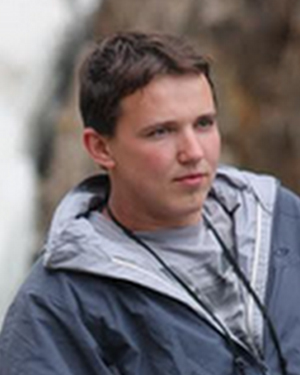
\includegraphics[width=1in,height
=1.25in,clip,keepaspectratio]{Photos_For_JSSC/PaulKlimov}}]{Paul Klimov} earned a Ph. D. from the University of Chicago in 2016, specializing in the quantum control of semiconductor spin qubits.  He joined Google AI Quantum in 2016, where he is currently a Senior Research Scientist working on optimizing superconducting qubit grids. 


\end{IEEEbiography}
\begin{IEEEbiography}[{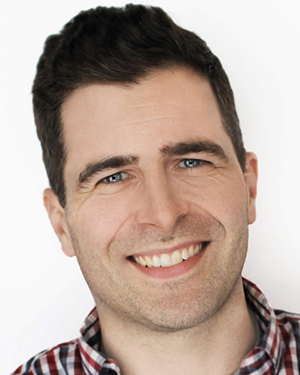
\includegraphics[width=1in,height
=1.25in,clip,keepaspectratio]{Photos_For_JSSC/josh}}]{Josh Mutus} received the PhD in Physics at the University of Alberta in Canada in 2012. He then joined the Quantum Computing group of John Martinis at the University of California Santa Barbara in 2012. He joined Google in 2014, where he currently serves as a senior research scientist within the AI Quantum group.


\end{IEEEbiography}
\begin{IEEEbiography}[{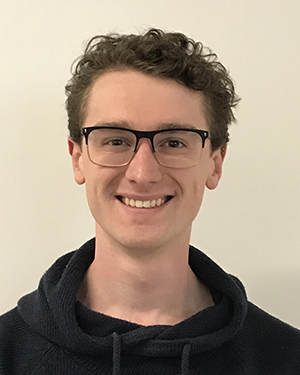
\includegraphics[width=1in,height
=1.25in,clip,keepaspectratio]{Photos_For_JSSC/MattMcEwen}}]{Matthew J. McEwen} received a Bachelor of Science (Physics) and Bachelor of Computer Engineering from the University of New South Wales, Australia in 2016. In 2018, he both joined the Google quantum hardware team and began a PhD in Physics at the University of California Santa Barbara.



\end{IEEEbiography}
\begin{IEEEbiography}[{\includegraphics[width=1in,height
=1.25in,clip,keepaspectratio]{Photos_For_JSSC/matthew}}]{Matthew Neeley} received a B.S. (2004) in physics from Stanford University and a Ph.D. (2010) in physics from the University of California, Santa Barbara, working on superconducting qubits. 

After graduate school he worked as a software engineer at Nest before joining the Google AI Quantum group to lead the Quantum OS team as a software engineer.


\end{IEEEbiography}
\begin{IEEEbiography}[{\includegraphics[width=1in,height
=1.25in,clip,keepaspectratio]{Photos_For_JSSC/charles}}]{Charles J. Neill} received a B.S. (2012) in physics from University of California, San Diego and a Ph.D. (2018) in physics from the University of California, Santa Barbara, studying  superconducting qubits. He joined Google AI Quantum as a research scientist in 2018, where he currently focuses on the calibration of multi-qubit systems and development of entangling gates.


\end{IEEEbiography}
\begin{IEEEbiography}[{\includegraphics[width=1in,height
=1.25in,clip,keepaspectratio]{Photos_For_JSSC/chris}}]{Chris Quintana} was born in Nyack, NY and graduated from Nyack high school in 2009. In 2013 he received his B.A. degree in physics (summa cum laude) from Princeton University, where he developed superconducting qubit and amplifier setups in the Petta lab. In 2017 he earned his Ph.D. in physics at UC Santa Barbara under John Martinis, working on flux noise and strong coupling of superconducting flux qubits. He currently works on multi-qubit devices in Google’s quantum hardware lab in Santa Barbara.


\end{IEEEbiography}
\begin{IEEEbiography}[{\includegraphics[width=1in,height
=1.25in,clip,keepaspectratio]{Photos_For_JSSC/Amit}}]{Amit Vainsencher}  received B.S. degrees in physics and mathematics from the University of California, Davis in 2008. In 2016, he earned his PhD in physics from the University of California, Santa Barbara on the topic of coupled piezoelectric and optical resonators.

Since 2016, he has been working as a research scientist at Google’s quantum computing hardware lab, focusing his efforts on scalable control electronics systems for quantum processors.

\end{IEEEbiography}
\begin{IEEEbiography}[{\includegraphics[width=1in,height
=1.25in,clip,keepaspectratio]{Photos_For_JSSC/Hartmut}}]{Hartmut Neven} received the PhD from the Institute for Neuroinformatics at the Ruhr University in Bochum, Germany in 1996.

He joined the University of Southern California as a Research Professor of Computer Science and Theoretical Neuroscience in 1998. He then founded two companies focused on computer vision. In 2006, his company,  Neven Vision, was acquired by Google, where he currently serves as an Engineering Director. He is the founder and manager of the Google Quantum Artificial Intelligence Lab, which aims to fabricate quantum processors and develop novel quantum algorithms to dramatically accelerate computational tasks for machine intelligence. Previously, he was head of the Google Visual Search team, where his team developed the visual search service that is used today by a large number of Google products including Image Search, Google Photos, YouTube, Street View, and Google Goggles. Hartmut was also a co-founder of project Glass and led the team that built the first prototype.

Dr. Neven has led teams that have won a number of competitions designed to establish the best visual recognition software for faces (FERET 1996, FRVT 2002), objects (ImageNet 2014) and text (ICDAR 2013).
\end{IEEEbiography}
\begin{IEEEbiography}[{\includegraphics[width=1in,height
=1.25in,clip,keepaspectratio]{Photos_For_JSSC/Martinis}}]{John Martinis} attended U.C. Berkeley from 1976 to 1987.  His PhD thesis was a pioneering demonstration of quantum-bit states in superconductors. After postdoctoral research at CEA in France, he joined NIST Boulder where he developed electron counting devices and x-ray microcalorimeters.  In 2004 he moved to U.C. Santa Barbara where he continued work on quantum computation.  In 2014 he was awarded the London Prize for low-temperature physics research.  In 2014 he joined the Google quantum-AI team to build a useful quantum computer. 

\end{IEEEbiography}
\end{document}